\documentclass[BufferStockTheory]{subfiles}% LaTeX path to the root directory of the current project, from the directory in which this file resides
% and path to econtexPaths which defines the rest of the paths like \FigDir
\providecommand{\econtexRoot}{}\renewcommand{\econtexRoot}{.}
\providecommand{\econtexPaths}{}\renewcommand{\econtexPaths}{\econtexRoot/Resources/econtexPaths}
% The \commands below are required to allow sharing of the same base code via Github between TeXLive on a local machine and Overleaf (which is a proxy for "a standard distribution of LaTeX").  This is an ugly solution to the requirement that custom LaTeX packages be accessible, and that Overleaf seems to ignore symbolic links (even if they are relative links to valid locations)
\providecommand{\econtex}{\econtexRoot/Resources/texmf-local/tex/latex/econtex}
\providecommand{\econtexSetup}{\econtexRoot/Resources/texmf-local/tex/latex/econtexSetup}
\providecommand{\econtexShortcuts}{\econtexRoot/Resources/texmf-local/tex/latex/econtexShortcuts}
\providecommand{\econtexBibMake}{\econtexRoot/Resources/texmf-local/tex/latex/econtexBibMake}
\providecommand{\econtexBibStyle}{\econtexRoot/Resources/texmf-local/bibtex/bst/econtex}
\providecommand{\econtexBib}{economics}
\providecommand{\notes}{\econtexRoot/Resources/texmf-local/tex/latex/handout}
\providecommand{\handoutSetup}{\econtexRoot/Resources/texmf-local/tex/latex/handoutSetup}
\providecommand{\handoutShortcuts}{\econtexRoot/Resources/texmf-local/tex/latex/handoutShortcuts}
\providecommand{\handoutBibMake}{\econtexRoot/Resources/texmf-local/tex/latex/handoutBibMake}
\providecommand{\handoutBibStyle}{\econtexRoot/Resources/texmf-local/bibtex/bst/handout}

\providecommand{\FigDir}{\econtexRoot/Figures}
\providecommand{\CodeDir}{\econtexRoot/Code}
\providecommand{\DataDir}{\econtexRoot/Data}
\providecommand{\SlideDir}{\econtexRoot/Slides}
\providecommand{\TableDir}{\econtexRoot/Tables}
\providecommand{\ApndxDir}{\econtexRoot/Appendices}

\providecommand{\ResourcesDir}{\econtexRoot/Resources}
\ifnum\pdfshellescape=1
\providecommand{\rootFromOut}{..} % Path back to root directory from output-directory
\providecommand{\LaTeXGenerated}{\econtexRoot/LaTeX} % Put generated files in subdirectory
\providecommand{\EqDir}{\econtexRoot/Equations} % Put generated files in subdirectory
\else
\providecommand{\rootFromOut}{.} % Path back to root directory 
\providecommand{\LaTeXGenerated}{\econtexRoot/} % Put generated files in main directory (because not allowed in subdirectory)
\providecommand{\EqDir}{\econtexRoot/} % Put generated files in main directory
\fi
\providecommand{\econtexPaths}{\econtexRoot/Resources/econtexPaths}
\providecommand{\LaTeXInputs}{\econtexRoot/Resources/LaTeXInputs}


% WARNING: Different execution depending on whether
% 0. Being compiled as standalone document
% * Compile this file, then main, then this one again
% * Keep iterating until neither file changes
% 0. Being compiled as subfile of main document

\onlyinsubfile{\externaldocument{BufferStockTheory}} % Get xrefs -- esp to appendix -- from main file; only works properly if main file has already been compiled; 

\begin{document}

\providecommand{\versn}{} % Version; like, web or pdf or journal submission
\ifthenelse{\boolean{ifWeb}}{  \renewcommand{\ushort}{\underline}\renewcommand{\versn}{Web} }{} % ushort does not work in tex4ht

% Put tiny info header at top to make it easy track git commit that generates it
\hfill{\tiny \jobname~\versn~\today~{at} \DTMcurrenttime, \input{\ResourcesDir/.git-source-commit}~~\input{\ResourcesDir/.git-public-commit}}

\title{Theoretical Foundations of \\ Buffer Stock Saving}

\author{Christopher D. Carroll\authNum}

\keywords{Precautionary saving, buffer stock saving, marginal propensity to consume, permanent income hypothesis}

\jelclass{D81, D91, E21\\
  \href{https://econ-ark.org}{\includegraphics{\ResourcesDir/PoweredByEconARK}}
}

\renewcommand{\forcedate}{October 19, 2020}
\date{\forcedate}

\maketitle 
\hypertarget{abstract}{}
\begin{abstract}
  This paper builds theoretical foundations for rigorous and intuitive understanding of `buffer stock' saving models, pairing each theoretical result with a quantitative exploration.  After describing conditions under which the consumption function exists, the paper shows that a `target' buffer stock exists only under conditions strictly stronger than those that guarantee convergence of the consumption and value functions.  Furthermore, the average growth rate of consumption equals the average growth rate of permanent income (in a small open economy populated by buffer stock savers).  Together, the (provided) numerical tools and (proven) analytical results constitute a comprehensive toolkit for understanding buffer stock models.
\end{abstract}

% Various resources 
\hypertarget{links}{}
\begin{footnotesize}
  \parbox{\textwidth}{
    \begin{center}
      \begin{tabbing}
        \texttt{Dashboard:~} \= \= \texttt{\href{https://econ-ark.org/materials/BufferStockTheory?dashboard}{https://econ-ark.org/materials/BufferStockTheory?dashboard}} \\
        \texttt{~~~~~~PDF:~} \> \> \texttt{\href{https://\owner.github.io/BufferStockTheory/BufferStockTheory.pdf}{https://\owner.github.io/BufferStockTheory/BufferStockTheory.pdf}} \\ % Owner is defined in BST preamble
        \texttt{~~~Slides:~} \> \> \texttt{\href{https://\owner.github.io/BufferStockTheory/BufferStockTheory-Slides.pdf}{https://\owner.github.io/BufferStockTheory/BufferStockTheory-Slides.pdf}} \\
        \texttt{~~~~~html:~} \> \> \texttt{\href{https://\owner.github.io/BufferStockTheory}{https://\owner.github.io/BufferStockTheory}}    \\
        \texttt{~Appendix:~} \> \> \texttt{\href{https://\owner.github.io/BufferStockTheory\#Appendices}{https://\owner.github.io/BufferStockTheory\#Appendices}}    \\
        \texttt{~~~bibtex:~} \> \> \texttt{\href{https://\owner.github.io/BufferStockTheory/LaTeX/BufferStockTheory-Self.bib}{https://\owner.github.io/BufferStockTheory/LaTeX/BufferStockTheory-Self.bib}}  \\
        \texttt{~~~GitHub:~} \> \> \texttt{\href{https://github.com/\owner/BufferStockTheory}{https://github.com/\owner/BufferStockTheory}} \\
      \end{tabbing}
    \end{center}
    
    The \href{https://econ-ark.org/materials/BufferStockTheory?dashboard}{dashboard} will launch a live interactive \href{https://en.wikipedia.org/wiki/Project\_Jupyter\#Jupyter_Notebook}{Jupyter Notebook} that uses the \href{https://econ-ark/HARK}{Econ-ARK/HARK} toolkit to produce all of the paper's figures (warning: the dashboard may take several minutes to launch).
  } % end parbox{\textwidth}
\end{footnotesize}

\begin{authorsinfo}
  \name{Contact: \href{mailto:ccarroll@jhu.edu}{\texttt{ccarroll@jhu.edu}}, Department of Economics, 590 Wyman Hall, Johns Hopkins University, Baltimore, MD 21218, \url{http://econ.jhu.edu/people/ccarroll}, and National Bureau of Economic Research.}
\end{authorsinfo}

\newcommand{\thankstext}{All figures and numerical results \href{https://econ-ark.github.io/nbreproduce}{can be automatically reproduced} using the \href{https://econ-ark/HARK}{Econ-ARK/HARK} toolkit, which can be cited per our references (\cite{carroll_et_al-proc-scipy-2018}); for reference to the toolkit itself see \href{https://econ-ark.org/acknowledging/}{Acknowleding Econ-ARK}.  Thanks to the \href{https://consumerfinance.gov}{Consumer Financial Protection Bureau} for funding the original creation of the \href{https://econ-ark.org}{Econ-ARK} toolkit; and to the \href{https://sloan.org}{Sloan Foundation} for funding Econ-ARK's \href{https://sloan.org/grant-detail/8071}{extensive further development} that brought it to the point where it could be used for this project.  The toolkit can be cited with its digital object identifier, \href{https://doi.org/10.5281/zenodo.1001067}{10.5281/zenodo.1001067}, as is done in the paper's own references as \cite{carroll_et_al-proc-scipy-2018}.  
  Thanks to James Feigenbaum, Joseph Kaboski, Miles Kimball, Qingyin Ma, Misuzu Otsuka, Damiano Sandri, John Stachurski, Adam Szeidl, Metin Uyanik, Mateo Vel\'asquez-Giraldo, Weifeng Wu, Xudong Zheng,  and Jiaxiong Yao for comments on earlier versions of this paper, John Boyd for help
  in applying his weighted contraction mapping theorem, Ryoji
  Hiraguchi for extraordinary mathematical insight that improved the
  paper greatly, David Zervos for early guidance to the literature,
  and participants in a seminar at Johns Hopkins University and a
  presentation at the 2009 meetings of the Society of Economic
  Dynamics for their insights.}

\ifthenelse{\boolean{ifWeb}}{}{\thanks{\thankstext}}

\titlepagefinish

% \begin{Web}
%   If web version, then just incorporate thanks at beginning of text
%   instead of in frontmatter
\ifthenelse{\boolean{ifWeb}}{\medskip \noindent {\tiny
    \thankstext \medskip \medskip \medskip
  }}{\pagebreak 
} % \end{Web}

% \begin{Web}
%   If web version, then just incorporate thanks at beginning of text
%   instead of in frontmatter
%   \ifthenelse{\boolean{ifWeb}}{\medskip \noindent {\tiny    \thankstext} \medskip \medskip \medskip \\    \noindent \hrule height 0.4pt depth 0.0pt width \textwidth \relax  }{\pagebreak } % \end{Web}

%   If web version, then just incorporate thanks at beginning of text instead of in frontmatter
\ifthenelse{\boolean{ifWeb}}{\medskip \noindent {\footnotesize \thankstext} \\  {\centering \medskip \medskip \medskip  \noindent \hrule height 0.4pt depth 0.0pt width \textwidth \relax}}{\pagebreak } % \end{Web}

\ifthenelse{\boolean{ifWeb}}{\thankstext}{}

\medskip \medskip

\hypertarget{Introduction}{}
\section{Introduction}

\label{sec:intro}

In the presence of empirically realistic transitory and permanent shocks to income \textit{a la} \cite{friedmanATheory}, only one further ingredient is required to construct a testable model of optimal consumption: A description of preferences.  Modelers usually assume geometric discounting of a constant relative risk aversion utility function, because, starting with Zeldes~\citeyearpar{zeldesStochastic} and Deaton~\citeyearpar{deatonLiqConstr}, a large literature has constructed numerical solutions whose quantitative predictions match microeconomic evidence reasonably well.

A companion theoretical literature has shown that numerical solution methods provide good approximations to limiting ``true'' mathematical solutions -- but only for models more complex than the simple case with just shocks and utility.  The extra complexity has been required because standard contraction mapping theorems (beginning with \cite{bellmanDynamicProgramming} and including those building on Stokey et.~al.~\citeyearpar{slpMethods}) cannot be applied when the utility function is unbounded (like CRRA - see \hyperlink{DiffFromLit}{section \ref{subsec:Setup}}).\footnote{It is unclear whether newer methods such as those of \cite{mnUnique} could overcome this problem, or how difficult it would be to do so; but in any case this particular problem does not seem to have been tackled by those methods or any others.}

This paper's first technical contribution is to articulate the (loose) conditions under which the simple problem (without convenient shortcuts like a consumption floor or liquidity constraints) defines a contraction mapping with a nondegenerate consumption function.  The interesting requirement is a \hyperlink{FVAC}{`Finite Value of Autarky'} condition.  The paper's second contribution is to specify the conditions under which the resulting consumption function implies existence of a `target' wealth-to-permanent-income ratio (the model exhibits `buffer stock' saving behavior).  Buffer stock behavior arises when the model's parameters satisfy a \hyperlink{GIC}{``Growth Impatience Condition''} (equation \eqref{eq:GIC}) that relates preferences and uncertainty to predictable income growth.

\hypertarget{KMP}{}

Even without a formal proof, target saving of this kind has been intuitively understood to underlie central quantitative results from the heterogeneous agent macroeconomics literature; for example, the logic of target saving is central to the explanation by \cite{kmpHandbook} of the fact that, during the Great Recession, middle-class consumers cut their consumption more than the poor or the rich.  The theoretical logic articulated below explains why:  Learning that the future has become more uncertain does not change the urgent imperatives of the poor (their high $\uFunc^{\prime}(\cRat)$ means they have little room to maneuver).  And, increased labor income uncertainty does not change the behavior of the rich because it does not threaten their consumption much.  Only people in the middle have both the motivation and the wiggle-room to reduce their discretionary spending.

Conveniently, elements required for the convergence proof also provide analytical foundations for many other results that have become familiar from the numerical literature.  In this paper, all theoretical conclusions are paired with numerically computed illustrations (using the open-source \href{https://econ-ark.org}{Econ-ARK} toolkit).  The insights of the paper are instantiated in the toolkit, whose \href{https://hark.readthedocs.io/en/stable/reference/ConsumptionSaving/ConsIndShockModel.html}{buffer stock saving module} algorithmically flags parametric choices under which a problem fails to define a contraction mapping; a target level of wealth does not exist; or the solution is otherwise surprising.

Such theoretical foundations are valuable both because they provide intuition about the determinants of saving targets, and because they make it easier to develop reliable numerical solution methods (by providing necessary and sufficient restrictions that solutions must satisfy).

The paper proceeds in three parts.

The first part articulates the \hyperlink{Sufficient-Conditions}{conditions required} for the problem to define a nondegenerate limiting consumption function, and explains how the paper's model is more general than those previously considered in the literature.  The conditions required for convergence are interestingly parallel to those required for the \hyperlink{Factors-Defined-And-Compared}{liquidity constrained perfect foresight model}; that parallel is explored and explained.  Next, the paper derives some limiting properties of the consumption function as resources (`cash') approach infinity and as they approach their lower bound; then the theorem is proven explaining when the problem defines a contraction mapping.  Finally, a related class of commonly-used models (exemplified by Deaton~\citeyearpar{deatonLiqConstr}) is shown to constitute a particular limit of this paper's model.

The \hyperlink{AnalysisoftheConvergedConsumptionFunction}{next section} examines five key properties of the model. First, as \hyperlink{LimitsAsmtToInfty}{cash approaches infinity} the expected growth rate of consumption and the marginal propensity to consume (MPC) converge to their values in the perfect foresight case. Second, as \hyperlink{LimitsAsmtToZero}{cash approaches zero} the expected growth rate of consumption approaches infinity, and the MPC approaches a simple analytical limit.  Third, if the consumer is `growth impatient,' a \hyperlink{onetarget}{unique target cash-to-permanent-income ratio} will exist.  Fourth, at the target cash ratio, the \hyperlink{cGroLTpGro}{expected growth rate of consumption} is slightly less than the expected growth rate of permanent (noncapital) income.  Finally, the expected growth rate of consumption \hyperlink{dcgdxneg}{is declining in the level of cash}. The first four propositions are proven under general assumptions about parameter values; the last is shown to hold if there are no transitory shocks, but may fail in extreme cases if there are both transitory and permanent shocks.

Szeidl~\citeyearpar{szeidlInvariant} has shown that such an economy will be characterized by stable invariant distributions for the consumption ratio, the wealth ratio, and other variables.\footnote{Szeidl's proof supplants the analysis in an earlier draft of this paper, which conjectured the result and provided supportive simulation evidence.}  Using Szeidl's result, the final section discusses conditions under which, even with a fixed aggregate interest rate that differs from the time preference rate, an economy populated by buffer stock consumers converges to a balanced growth equilibrium in which the growth rate of consumption tends toward the (exogenous) growth rate of permanent income.

\hypertarget{The-Problem}{}
\section{The Problem}

\subsection{Setup}
\label{subsec:Setup}

The consumer solves a standard optimization problem from the current period $t$ until the end of life at $T$: 
\begin{verbatimwrite}{\EqDir/supfn.tex}
  \begin{align*}%    \label{eq:supfn}
    \max~ \Ex_{t}\left[\sum_{n=0}^{T-t} \DiscFac^{n} \uFunc(\cLevBF_{t+n})\right]
  \end{align*}
\end{verbatimwrite}
  \begin{align*}%    \label{eq:supfn}
    \max~ \Ex_{t}\left[\sum_{i=0}^{n} \DiscFac^{i} \uFunc(\cLevBF_{t+i})\right]
  \end{align*}

where
\begin{align}
  \uFunc(\bullet)=\bullet^{1-\CRRA}/(1-\CRRA) \label{eq:crrautil}
\end{align}
is a constant relative risk aversion utility function with $\CRRA > 1$.\footnote{The main
  results also hold for logarithmic utility which is the limit as
  $\CRRA \rightarrow 1$ but incorporating the logarithmic special case
  in the proofs is cumbersome and therefore
  omitted.}$^{,}$\footnote{We will define the infinite horizon
  solution as the limit of the finite horizon problem as the horizon
  $T-t$ approaches infinity.}  The consumer's initial condition is
defined by market resources $\mLevBF_{t}$ (\cite{deatonLiqConstr}'s
`cash-on-hand') and permanent noncapital income $\pLevBF_{t}$.

In the usual treatment, a dynamic budget constraint (DBC) incorporates
several different elements that determine next period's $\mLevBF$ (given this
period's choices); but for the detailed analysis here, it will be useful to
disarticulate the steps so that individual ingredients can be separately examined:
\begin{verbatimwrite}{\EqDir/DBCparts.tex}
  \begin{align}
    \aLevBF_{t}    & = \mLevBF_{t}-\cLevBF_{t}  \label{eq:DBCparts} \\
    \bLevBF_{t+1}    & = \aLevBF_{t} \Rfree \notag \\
    \pLevBF_{t+1}  & = \pLevBF_{t} \underbrace{\PGro\pShk_{t+1}}_{\equiv \PGro_{t+1}}  \notag \\
    \mLevBF_{t+1}  & =  \bLevBF_{t+1} +\pLevBF_{t+1}\tShkAll_{t+1},  \notag
  \end{align}
\end{verbatimwrite}
  \begin{align}
    \aLevBF_{t}    & = \mLevBF_{t}-\cLevBF_{t}  \label{eq:DBCparts} \\
    \bLevBF_{t+1}    & = \aLevBF_{t} \Rfree \notag \\
    \pLevBF_{t+1}  & = \pLevBF_{t} \underbrace{\PGro\pShk_{t+1}}_{\equiv \PGro_{t+1}}  \notag \\
    \mLevBF_{t+1}  & =  \bLevBF_{t+1} +\pLevBF_{t+1}\tShkAll<_{t+1},  \notag
  \end{align}
 where $\aLevBF_{t}$ indicates the consumer's assets at the end of period $t$, which grow by a fixed interest factor $\Rfree =(1+\rfree)$ between periods,\footnote{See \cite{mstCapIncFluct} for interesting new work that considers the case where capital returns are stochastic and liquidity constraints exist.  \cite{benhabibWealth} examines implications of capital income risk for the distribution of wealth.}  so that $\bLevBF_{t+1}$ is the consumer's financial (`bank') balances before next period's consumption choice;\footnote{Allowing a stochastic interest factor is straightforward but adds little insight.%  The effects are more interesting for analysis of the invariant distribution (\cite{szeidlInvariant}).
} $\mLevBF_{t+1}$ (`market resources' or `money') is the sum of financial wealth $\bLevBF_{t+1}$ and noncapital income $\pLevBF_{t+1}\tShkAll_{t+1}$ (permanent noncapital income $\pLevBF_{t+1}$ multiplied by a mean-one iid transitory income shock factor $\tShkAll_{t+1}$; future transitory shocks are assumed to satisfy $\Ex_{t}[{\tShkAll}_{t+n}]=1~\forall~n\geq 1$). Permanent noncapital income in period $t+1$ is equal to its previous value, multiplied by a growth factor $\PGro$, modified by a mean-one iid shock $\pShk_{t+1}$, $\Ex_{t}[{\pShk}_{t+n}]=1~\forall~n \geq 1$ satisfying $\pShk \in [\ushort{\pShk},\bar{\pShk}]$ for $0 < \ushort{\pShk} \leq 1 \leq \bar{\pShk} < \infty$ (and $\ushort{\pShk}=\bar{\pShk}=1$ is the degenerate case with no permanent shocks).\footnote{It is useful to emphasize that permanent noncapital income as defined here differs from what Deaton~\citeyearpar{deatonUnderstandingC} calls permanent income (which is often adopted in the macro literature).  Deaton defines permanent income as the amount that a perfect foresight consumer could spend while leaving total (human and nonhuman) wealth constant.  Relatedly, we refer to $\mLevBF_{t}$ as `cash-on-hand' or `market resources' rather than as wealth to avoid any confusion for readers accustomed to thinking of the discounted value of future noncapital income as a part of wealth.  The `market resources' terminology is motivated by the model's assumption that human wealth cannot be capitalized, an implication of anti-slavery laws.}$^{,}$\footnote{Hereafter for brevity we occasionally drop time subscripts, e.g.\ $\Ex[\pShk^{-\CRRA}]$ signifies $\Ex_{t}[\pShk_{t+1}^{-\CRRA}]$.}

In future periods $t+n ~\forall~ n \geq 1$ there is a small probability $\pZero$ that income will
be zero (a `zero-income event'),
\begin{verbatimwrite}{\EqDir/tShkDef}
  \begin{equation}
    \tShkAll _{t+n}=
    \begin{cases}
      0\phantom{_{t+1}/\pNotZero} & \text{with probability $\pZero>0$} \\
      \tShkEmp_{t+n}/\pNotZero      & \text{with probability $\pNotZero  $} % \equiv (1-\pZero) 
    \end{cases} \label{eq:tShkDef}
  \end{equation}
\end{verbatimwrite}
  \begin{equation}
    \tShkAll _{t+n}=
    \begin{cases}
      0\phantom{_{t+1}/\pNotZero} & \text{with probability $\pZero>0$} \\
      \tShkEmp_{t+n}/\pNotZero      & \text{with probability $\pNotZero  $} % \equiv (1-\pZero)
    \end{cases} \label{eq:tShkDef}
  \end{equation}

where $\tShkEmp_{t+n}$ is an iid mean-one random variable
($\Ex_{t}[{\tShkEmp}_{t+n}]=1~\forall~n>0$)
with a distribution
satisfying $\tShkEmp \in \lbrack \ushort{\tShkEmp},\bar{\tShkEmp}\rbrack$
where $0<\ushort{\tShkEmp} \leq 1 \leq \bar{\tShkEmp}<\infty$
(degenerately $\ushort{\tShkEmp}=\bar{\tShkEmp}=1$).\footnote{See \cite{rabaultBorrowing} and \cite{lsIncFluct} for analyses of cases where the shock processes have unbounded support.}  Call the cumulative
distribution functions $\CDF_{\pShk}$ and $\CDF_{\tShkEmp}$ (where $\CDF_{\tShkAll}$
is derived trivially from \eqref{eq:tShkDef} and $\CDF_{\tShkEmp}$).
Permanent income and cash start out strictly positive, $\{\pLevBF_{t},\mLevBF_{t}\} \in
(0,\infty)$, and as usual the consumer cannot die in
debt, so
\begin{align}
  \cLevBF_{T} & \leq  \mLevBF_{T} \label{eq:NoDebtAtDeath}.
\end{align}

\hypertarget{PDV}{}
The model looks more special than it is.  In particular, the
assumption of a positive probability of zero-income events may seem
objectionable.  However, it is easy to show that a model with a
nonzero minimum value of $\tShkAll$ (motivated, for example, by the
existence of unemployment insurance) can be redefined by capitalizing
the present discounted value of minimum income into current market assets,\footnote{So long
  as this PDV is a finite number and unemployment benefits are
  proportional to $\pLevBF_{t}$; see the discussion in
  section~\ref{sec:discussConvergence}.}  analytically transforming
that model back into the model analyzed here.  Also, the assumption of
a positive point mass (as opposed to positive density) for the worst
realization of the transitory shock is inessential, but simplifies the proofs and is a powerful aid to intuition.\footnote{No key results would change if the unemployment state were persistent but mean-reverting, instead of IID.}

\begin{comment}
  Combining the transition equations, the recursive nature of
  the problem allows us to rewrite it more compactly in Bellman equation form,
  \begin{align*}
    \VFunc_{t}(\mLevBF_{t},\pLevBF_{t})  & = \max_{\cLevBF_{t}}~\left\{\uFunc(\cLevBF_{t})+\DiscFac \Ex_{t}\left[ \VFunc_{t+1}((\mLevBF_{t}-\cLevBF_{t})\Rfree+ \pLevBF_{t+1}\tShkAll_{t+1},\pLevBF_{t} \PGro  \pShk_{t+1})\right]\right\}
                                           .
  \end{align*}
\end{comment}

\hypertarget{DiffWithLit}{} This model differs from Bewley's~\citeyearpar{bewleyPIH} classic formulation in several ways. The CRRA utility function does not satisfy Bewley's assumption that $\uFunc(0)$ is well defined, or that $\uP(0)$ is well defined and finite; indeed, neither the value function nor the marginal value function will be bounded.  It differs from Schectman and Escudero~\citeyearpar{seIncFluct} in that they impose liquidity constraints and positive minimum income.  It differs from both of these in that it permits permanent growth in income, and also permanent shocks to income, which a large empirical literature finds are quantitatively important in micro data\footnote{MaCurdy~\citeyearpar{macurdyTimeseries}; Abowd and Card~\citeyearpar{acCovariance}; Carroll and Samwick~\citeyearpar{csNature}; Jappelli and Pistaferri~\citeyearpar{jpCins}; Storesletten, Telmer, and Yaron~\citeyearpar{styConsumption}; \cite{blpRisk}} and which since~\cite{friedmanATheory} have been understood to be far more consequential for household welfare than are transitory fluctuations.  It differs from Deaton~\citeyearpar{deatonLiqConstr} because liquidity constraints are absent; there are separate transitory and permanent shocks ({\it a la} \cite{muthOptimal}); and the transitory shocks here can occasionally cause income to reach zero.\footnote{Below it will become clear that the Deaton model is a particular limit of this paper's model.}  Finally, it differs from models found in Stokey et.\ al.~\citeyearpar{slpMethods} because neither liquidity constraints nor bounds on utility or marginal utility are imposed.\footnote{Similar restrictions to those in the cited literature are made in the well known papers by Scheinkman and Weiss~\citeyearpar{scheinkman&weiss:borrowing} and Clarida~\citeyearpar{claridaErgodic}.  See \cite{tocheUrisk} for an elegant analysis of a related but simpler continuous-time model.}$^{,}$\footnote{\cite{asHomogeneous} relaxed the bounds on the return function, but they address only the deterministic case.}

The incorporation of permanent shocks rules out application of the tools of \cite{mnUnique}, who followed and corrected an error in the fundamental work on the local contraction mapping method developed in \cite{rrExistence}.  \cite{mvExistence} provides a correction to \cite{rrExistence}, and provides conditions that are easier to verify, but again only addresses the deterministic case.  

\hypertarget{The-Problem-Can-Be-Rewritten-in-Ratio-Form}{}
\subsection{The Problem Can Be Rewritten in Ratio Form}

\label{subsec:ratio}

We establish a bit more notation by reviewing the standard result that in problems of this class (CRRA utility, permanent shocks) the number of relevant state variables can be reduced from two ($\mLevBF$ and $\pLevBF$) to one $(\mRat = \mLevBF/\pLevBF)$.  Generically defining nonbold variables as the boldface counterpart normalized by $\pLevBF_{t}$ (as with $\mRat$), assume that value in the last period of life is $\uFunc(\mLevBF_{T})$, and consider the problem in the second-to-last period,
\begin{align}
  \vLevBF_{T-1}(\mLevBF_{T-1},\pLevBF_{T-1})  & = 
                                                \max_{\cLevBF_{T-1}}~ \uFunc(\cLevBF_{T-1}) +\DiscFac \Ex_{T-1} [ \uFunc(\mLevBF_{T})]
                                                \notag \\
                                              & =  \max_{\cRat_{T-1}}~
                                                \uFunc(\pLevBF_{T-1}\cRat_{T-1}) + \DiscFac  \Ex_{T-1} [\uFunc(\pLevBF_{T}{\mRat}
                                                _{T})]  \notag \\
                                              & = \pLevBF_{T-1}^{1-\CRRA}
                                                \left\{\max_{\cRat_{T-1}}~ \uFunc(c_{T-1}) + \DiscFac \Ex_{T-1} [ \uFunc( {\PGro}_{T}
                                                {\mRat}_{T}) ] \right\},   \label{eq:vBold}
\end{align}
where the last line follows because for the CRRA utility function \eqref{eq:crrautil}, $\uFunc(xy) =
x^{1-\CRRA}\uFunc(y)$.

\hypertarget{The-Related-Problem}{}
Now, in a one-time deviation from the notational convention established in the last paragraph, define nonbold `normalized value' not as $\vLevBF_{t}/\pLevBF_{t}$ but as $\vFunc_{t} = \vLevBF_{t}/\pLevBF_{t}^{1-\CRRA}$, because this allows us to exploit features of the related problem,
\begin{align}
  \vFunc_{t}(\mRat_{t})  & = \max_{\{\cFunc\}_{t}^{T}}~  \uFunc(\cFunc_{t}) +\DiscFac \Ex_{t}[\PGro_{t+1}^{1-\CRRA}\vFunc_{t+1}({\mRat}_{t+1})] \notag \\
                         & \mbox{s.t.}  \label{eq:veqn} 
  \\ {\aRat}_{t}  & = \mRat_{t}-c_{t}  \notag
  \\ {\bRat}_{t+1}  & = (\Rfree/\PGro_{t+1})\aRat_{t}  ~ = ~ \Rnorm_{t+1}\aRat_{t}  \notag
  \\ \mRat_{t+1}  & = \bRat_{t+1}+\tShkAll_{t+1}  \notag, %
\end{align}
where $\Rnorm_{t+1}\equiv (\Rfree/\PGro_{t+1})$ is a `growth-normalized' return factor, and the new problem's first order condition is
\begin{align}
  c_{t}^{-\CRRA}  & = \Rfree \DiscFac \Ex_{t}[ {\PGro}_{t+1}^{-\CRRA} {\cRat}
                    _{t+1}^{-\CRRA}].  \label{eq:scaledeuler}
\end{align}

Since $\vFunc_{T}(\mRat_{T}) = \uFunc(\mRat_{T})$, defining $\vFunc_{T-1}(\mRat_{T-1})$ from \eqref{eq:veqn}, we obtain
\begin{align*}
  \vLevBF_{T-1}(\mLevBF_{T-1},\pLevBF_{T-1})  & = \pLevBF_{T-1}^{1-\CRRA} \vFunc_{T-1}(\underbrace{\mLevBF_{T-1}/\pLevBF_{T-1}}_{=\mRat_{T-1}}).
\end{align*}

This logic induces to all earlier periods, so that if we solve the
normalized one-state-variable problem \eqref{eq:veqn}, we
will have solutions to the original problem for any $t<T$
from:
\begin{align*}
  \vLevBF_{t}(\mLevBF_{t},\pLevBF_{t})  & = \pLevBF_{t}^{1-\CRRA}\vFunc_{t}(\mRat_{t}),
  \\ \cLevBF_{t}(\mLevBF_{t},\pLevBF_{t})  & = \pLevBF_{t}\cFunc_{t}(\mRat_{t}).
\end{align*}

\hypertarget{Definition-of-a-Nondegenerate-Solution}{}
\subsection{Definition of a Nondegenerate Solution}

We say that this problem has a nondegenerate solution if, as the number of remaining periods of life gets arbitrarily large, the backward-iterating solution defines a unique limiting consumption function $\cRat(\bullet)$ that satisfies
\begin{align}
  0 & < \cRat(\mRat) <  \infty 
\end{align}
for every $0 < \mRat < \infty.$ (`Degenerate' limits will be cases
where the limiting consumption function is $\cFunc(\mRat)=0$ or $\cFunc(\mRat)=\infty$.)

\hypertarget{Perfect-Foresight-Benchmarks}{}
\subsection{Perfect Foresight Benchmarks}

The familiar analytical solution to the perfect foresight specialization of the model, obtained by setting $\pZero=0$ and $\ushort{\tShkEmp}=\bar{\tShkEmp}=\ushort{\pShk}=\bar{\pShk}=1$, allows us to define some remaining notation and terminology.

\hypertarget{Human-Wealth}{}
\subsubsection{Human Wealth}
The dynamic budget constraint, strictly positive marginal utility, and the can't-die-in-debt condition \eqref{eq:NoDebtAtDeath} imply an exactly-holding intertemporal budget constraint (IBC):
\begin{align}
  \text{PDV}_{t}(\cLevBF)  & = \overbrace{\mLevBF_{t}-\pLevBF_{t}}^{\bLevBF_{t}}+\overbrace{\text{PDV}_{t}(\pLevBF)}^{\hLevBF_{t}}, \label{eq:IBCFinite}
\end{align}
where $\bLevBF$ is nonhuman wealth and $\hLevBF_{t}$ is `human wealth,' and with a constant $\Rnorm \equiv \Rfree/\PGro$,
\begin{align}
  \hLevBF_{t}  & = \pLevBF_{t}+\Rnorm^{-1} \pLevBF_{t} + \Rnorm^{-2} \pLevBF_{t} + ... + \Rnorm^{t-T} \pLevBF_{t} \label{eq:HDef}
  \\  & = \underbrace{\left(\frac{1-\Rnorm^{-(T-t+1)}}{1-\Rnorm^{-1}}\right)}_{\equiv \hRat_{t}}\pLevBF_{t} .
\end{align}
This equation shows that in order for $\hRat \equiv \lim_{n \rightarrow
  \infty} \hRat_{T-n}$ to be finite, we must
impose the Finite Human Wealth Condition (`\FHWC'): \hypertarget{FHWC}{}
\begin{align}
  \underbrace{\PGro/\Rfree}_{\equiv \Rnorm^{-1}}  & < 1 \label{eq:FHWC}.
\end{align}
Intuitively, for human wealth to be finite, the growth rate of (noncapital) income must be smaller than
the interest rate at which that income is being discounted.

\hypertarget{Unconstrained-Solution}{}
\subsubsection{Unconstrained Solution} \label{subsec:PFUncon}

\hypertarget{APF}{}
\hypertarget{AIC}{}
The consumption Euler equation holds in every period; with $\uP(\cLevBF)=\cLevBF^{-\CRRA}$, \hypertarget{Pat}{}
\begin{align}
  \cLevBF_{t+1}/\cLevBF_{t}  & = (\Rfree\DiscFac)^{1/\CRRA} \equiv \Pat   \label{eq:Pat}
\end{align}
where the Old English letter `thorn' represents what we will call the
`absolute patience factor' $(\Rfree
\DiscFac)^{1/\CRRA}$.\footnote{Impatience conditions of one kind or
  another have figured in intertemporal optimization problems since
  such problems were first formalized in economics, most notably by \cite{ramseySave}.
  Discussion of these issues was prominent in the literature of the
  1960s and 1970s, and no brief citations here could do justice to the literature on the topic, so I refrain from the attempt.}  The sense in which $\Pat$ captures
patience is that if the `absolute impatience condition' (\AIC) holds,
\begin{align}
  \label{eq:AIC}
  \Pat  & < 1,
\end{align}
the consumer will choose to spend an amount too large to sustain indefinitely (the
level of consumption must fall over time).  We call such a consumer `absolutely impatient' (the key condition in \cite{bewleyPIH}).

We next define a `return patience factor' that relates absolute patience to the return factor:
\begin{align}
  \PatR  & \equiv  {\Pat}/\Rfree \label{eq:PatR}
\end{align}
and since consumption is growing by $\Pat$ but discounted by $\Rfree$:
\begin{align}
  \text{PDV}_{t}(\cLevBF)  & = \left(1+\PatR+\PatR^{2}+...+ \PatR^{T-t}\right)\cLevBF_{t} \notag
  \\  & = \left(\frac{1-\PatR^{T-t+1}}{1-\PatR}\right)\cLevBF_{t}
\end{align}
from which the IBC \eqref{eq:IBCFinite} implies
\begin{align}
  \cLevBF_{t}  & = \overbrace{\left(\frac{1-\PatR}{1-\PatR^{T-t+1}}\right)}^{\equiv \MinMPC_{t}}
                 (\bLevBF_{t}+\hLevBF_{t})   \label{eq:WDef}
\end{align}
which defines a normalized finite-horizon perfect foresight consumption function
\begin{align}
  \bar{\cFunc}_{T-n}(\mRat_{T-n})  & = (\overbrace{\mRat_{T-n}-1}^{
                                     \equiv\bRat_{T-n}}+\hRat_{T-n})\MinMPC_{T-n}
\end{align}
where $\MinMPC_{t}$ is the marginal propensity to consume (MPC) because it answers the
question `if the consumer had an extra unit of wealth, how much more would be spent.' \hypertarget{RIC}{}
(The overbar on $\cFunc$ reflects the fact that this will be an upper bound as we modify the problem to incorporate constraints and uncertainty; analogously, the underbar for $\MPC$ indicates that it is a lower bound).
Equation \eqref{eq:WDef} makes plain that for the limiting
MPC to be strictly positive as $n=T-t$ goes to infinity we must impose the Return Impatience Condition (\RIC):
\begin{align}
  \PatR  & < 1   \label{eq:RIC},
\end{align}
so that
\begin{align}
  0 <  \MinMPC  & \equiv   1-\PatR = \lim_{n \rightarrow \infty} \MinMPC_{T-n} \label{eq:MinMPCDef}
                  .
\end{align}

The {\RIC} thus imposes a second kind of `impatience:' The consumer cannot be so pathologically patient as to wish, in the limit as the horizon approaches infinity, to spend nothing today out of an increase in current wealth; that is, the condition rules out the degenerate limiting solution $\bar{\cFunc}(\mRat)=0$.  Because the return patience factor $\PatR$ is the absolute patience factor divided by the return, we call equation \eqref{eq:RIC} the `return impatience condition' or \RIC; we will say that a consumer who satisfies the condition is `return impatient.'

Given that the {\RIC}~holds, and defining limiting objects by the absence of a time subscript (e.g., $\bar{\cFunc}(\mRat)=\lim_{n \uparrow \infty} \bar{\cFunc}_{T-n}(\mRat)$), the limiting consumption function will be
\begin{align}\label{eq:cFuncPFUnc}
  \bar{\cFunc}(\mRat)  & = (\mRat+\hRat-1)\MinMPC, 
\end{align}
and we now see that in order to rule out the degenerate limiting
solution $\bar{\cFunc}(\mRat) = \infty$ we need $\hRat$ to be finite; that is, we
must impose the finite human wealth condition \eqref{eq:FHWC}.

\hypertarget{ValuePFAnalytical}{}
A final useful point is that since the perfect foresight
growth factor for consumption is $\Pat$, $\uFunc(xy) =
x^{1-\CRRA}\uFunc(y)$ yields an analytical expression for value:  
\begin{align}
  \vRat_{t}  & = \uFunc(\cRat_{t})+\DiscFac \uFunc(\cRat_{t}\Pat)+\DiscFac^{2} \uFunc(\cRat_{t} \Pat^{2})+... \label{eq:ValuePFAnalytical}
  \\  & = \uFunc(\cRat_{t})\left(1+\DiscFac \Pat^{1-\CRRA}+(\DiscFac \Pat^{1-\CRRA})^{2}+...\right) \notag 
  \\  & = \uFunc(\cRat_{t})\left(\frac{1-(\DiscFac \Pat^{1-\CRRA})^{T-t+1}}{1-\DiscFac \Pat^{1-\CRRA}}\right) \notag
\end{align}
which asymptotes to a finite number as $n=T-t$ approaches $+\infty$ if $\DiscFac \Pat^{1-\CRRA} < 1;$\footnote{This is related to a condition in \cite{asHomogeneous}.} with a bit of algebra,\footnote{
  \begin{align*}
    \DiscFac ((\Rfree \DiscFac)^{1/\CRRA})^{1-\CRRA}  & < 1
    \\ \DiscFac (\Rfree\DiscFac)^{1/\CRRA}/\Rfree\DiscFac  & < 1
    \\ (\Rfree \DiscFac)^{1/\CRRA} /\Rfree  & < 1
  \end{align*}.
} this requirement can be shown to be equivalent to the {\RIC}.  Thus, the same conditions that guarantee a nondegenerate limiting consumption function also guarantee a nondegenerate limiting value function (which, interestingly, will \textit{not} be true when we incorporate uncertainty).

\hypertarget{Constrained-Solution}{}
\subsubsection{Constrained Solution}

If a liquidity constraint requiring $\bRat \geq 0$ is ever to be relevant, it must be
relevant at the lowest possible level of market resources,
$\mRat_{t}=1$, which obtains for a consumer who enters period $t$ with
$\bRat_{t}=0$.  The constraint is `relevant' if
it prevents the choice that would otherwise be optimal; at
$\mRat_{t}=1$ the constraint is relevant if the marginal utility from spending all of today's
resources $c_{t}=m_{t}=1$, exceeds the marginal utility from
doing the same thing next period, $\cRat_{t+1}=1$; that is, if such
choices would violate the Euler equation \eqref{eq:scaledeuler}:
\begin{align}
  1^{-\CRRA}  & > \Rfree \DiscFac (\PGro)^{-\CRRA}1^{-\CRRA}  \label{eq:LiqConstrBinds}.
\end{align}

\hypertarget{PFGPF}{}
\hypertarget{PFGIC}{}
By analogy to the return patience factor, we therefore define a `perfect
foresight growth patience factor' (\PFGPF) as
\begin{align}
  \PatPGro  & = {\Pat}/\PGro,  \label{eq:PFGPF}
\end{align}
and define a `perfect foresight growth impatience condition' (\PFGIC)
\begin{align}
  \label{eq:PFGIC}
  \PatPGro &  < 1
\end{align}
which is equivalent to \eqref{eq:LiqConstrBinds} (exponentiate both
sides by $1/\CRRA$).

If the \RIC~\eqref{eq:RIC} and the \FHWC~\eqref{eq:FHWC} hold, appendix \ref{sec:ApndxLiqConstr} shows
that, for some $0 < \mRat_{\#} < 1$, an unconstrained consumer behaving according to
\eqref{eq:cFuncPFUnc} would choose $\cRat < \mRat$ for all $\mRat >
\mRat_{\#}$.  In this case the solution to the constrained consumer's problem is simple: For any $\mRat
\geq \mRat_{\#}$ the constraint does not bind (and will never bind in
the future) so the constrained consumption function is identical
to the unconstrained one.  If the consumer were somehow\footnote{``Somehow'' because $\mRat<1$ could only be
  obtained by entering the period with $\bRat < 0$ which the constraint
  forbids.}
to arrive at an $\mRat < \mRat_{\#} < 1$ the constraint would bind and
the consumer would have to consume $\cRat=\mRat$.  The $\circ$ accent will designate the limiting
constrained consumption function:
\begin{equation}
  \mathring{\cFunc}(\mRat)=
  \begin{cases}
    \mRat & \text{if $\mRat < \mRat_{\#}$} \\
    \bar{\cFunc}(\mRat)  & \text{if $\mRat \geq \mRat_{\#}$.}
  \end{cases}
\end{equation}

More useful is the case where the perfect foresight growth and return impatience conditions both hold.  In this case appendix \ref{sec:ApndxLiqConstr} shows that the limiting constrained consumption function is piecewise linear, with $\mathring{\cFunc}(\mRat)=\mRat$ up to a first `kink point' at $\mRat_{\#}^{1}>1$, and with discrete declines in the MPC at a set of kink points $\{\mRat_{\#}^{1},\mRat_{\#}^{2},...\}$.  As $\mRat \uparrow \infty$ the constrained consumption function $\mathring{\cFunc}(\mRat)$ becomes arbitrarily close to the unconstrained $\bar{\cFunc}(\mRat)$, and the marginal propensity to consume function $\mathring{\MPCFunc}(\mRat) \equiv \mathring{\cFunc}^{\prime}(\mRat)$ limits to $\MinMPC$.  Similarly, the value function $\mathring{\vFunc}(\mRat)$ is nondegenerate and limits into the value function of the unconstrained consumer.  This logic holds even when the finite human wealth condition fails (denoted \cncl{\FHWC}):  A solution exists because the constraint prevents the consumer from borrowing against infinite human wealth to finance infinite current consumption.  Under these circumstances, the consumer who starts with any amount of resources $\bRat_{t} > 1$ will, over time, run those resources down so that by some finite number of periods $n$ in the future the consumer will reach $\bRat_{t+n} = 0$, and thereafter will set $\cRat = \mRat = 1$ for eternity, a policy that will (using \eqref{eq:ValuePFAnalytical}) yield value of \hypertarget{PFFVAC}{}
\begin{align}
  \vLevBF_{t+n}  & = \uFunc(\pLevBF_{t+n})\left(1+\DiscFac
                   \PGro^{1-\CRRA}+(\DiscFac \PGro^{1-\CRRA})^{2}+...\right) \notag
  \\  & = \PGro^{n(1-\CRRA)} \uFunc(\pLevBF_{t})\left(\frac{1-(\DiscFac
        \PGro^{1-\CRRA})^{T-(t+n)+1}}{1-\DiscFac \PGro^{1-\CRRA}}\right),
        \notag
\end{align}
which will be finite whenever 
\begin{align}
  \overbrace{\DiscFac \PGro^{1-\CRRA} }^{\equiv \DiscAlt}  & < 1 \nonumber
  \\ \DiscFac \Rfree \PGro^{-\CRRA}  & < \Rfree/\PGro \label{eq:PFFVAC} 
  \\ \PatPGro  & < (\Rfree/\PGro)^{1/\CRRA}, \nonumber
\end{align}
which we call the Perfect Foresight Finite Value of Autarky Condition, \PFFVAC, because it guarantees that a consumer who always spends all permanent income will have finite value (the consumer has `finite autarky value').  Note that the version of the \PFFVAC~in \eqref{eq:PFFVAC} implies the \PFGIC~$\PatPGro < 1$ whenever \cncl{\FHWC} ($\Rfree < \PGro$) holds.  So, if \cncl{\FHWC}, value for any finite $\mRat$ will be the sum of two finite numbers: The component due to the unconstrained consumption choice made over the finite horizon leading up to $\bRat_{t+n} = 0$, and the finite component due to the value of consuming all $\pLevBF_{t+n}$ thereafter.  The consumer's value function is therefore nondegenerate.

\hypertarget{RICandFHWCFail}{}
The most peculiar possibility occurs when the \RIC~fails.  Under these circumstances the \FHWC~must also fail (Appendix~\ref{sec:ApndxLiqConstr}), and the constrained consumption function is nondegenerate.  (See appendix Figure~\ref{fig:PFGICHoldsFHWCFailsRICFails} for a numerical example).  While it is true that $\lim_{m \uparrow \infty}
\mathring{\MPCFunc}(\mRat) = 0$, nevertheless the limiting constrained
consumption function $\mathring{\cFunc}(\mRat)$ is strictly positive
and strictly increasing in $\mRat$.  This result interestingly
reconciles the conflicting intuitions from the unconstrained case,
where \cncl{\RIC} would suggest a degenerate limit of
$\mathring{\cFunc}(\mRat)=0$ while \cncl{\FHWC} would suggest a
degenerate limit of $\mathring{\cFunc}(\mRat)=\infty$.

Table~\ref{table:Comparison} and \ref{table:Required} (and appendix table~\ref{table:LiqConstrScenarios}) codify the key points to help the reader keep them straight.

An intuitive representation of the relations of the conditions is presented in Figure~\ref{fig:RelatePFGICFHWCRICPFFVAC} (for the perfect foresight case).  Each node represents a quantity considered in the foregoing analysis.  The arrow associated with each inequality condition reflects the imposition of that condition.  For example, one way of writing the {\PFFVAC} is $\Pat < \Rfree^{1/\CRRA} \PGro^{1-1/\CRRA}$, and this is captured by the diagonal arrow.  Traversing the diagram clockwise starting at $\Pat$ involves imposing first the {\PFGIC} then the {\FHWC}, and the consequent arrival at the bottom right node tells us that these two conditions jointly imply that the {\PFFVAC} holds.  Reversal of a condition will reverse the arrow's direction; so, for example, {\cncl{\FHWC}} would correspond to reversing the directon of the bottommost arrow.  This would allow us to follow the arrows in a counterclockwise direction from $\Pat$ to the bottom right node, leading to the conclusion that the combination of {\RIC} and \cncl{\FHWC} implies that the {\PFFVAC} holds.  (Readers unfamiliar with diagrams of this kind may wish to consult the expanded discussion in Appendix~\ref{sec:ApndxConditionDiagrams}).

\providecommand{\figName}{RelatePFGICFHWCRICPFFVAC} % Allows generic definition of hypertargets based on title of figure
\providecommand{\figFile}{\figName} %  and on filename
\hypertarget{\figFile}{}
\hypertarget{\figName}{}
\input{\FigDir/\figName} % Read in the tex to generate the figure

We now turn to the case with uncertainty.  The model without constraints but with uncertainty will turn out to be a close parallel to the model with constraints but without uncertainty.

\hypertarget{Uncertainty-Modified-Conditions}{}
\subsection{Uncertainty-Modified Conditions}
\subsubsection{Impatience}

When uncertainty is introduced, the expectation of $\bRat_{t+1}$ can be rewritten as:  
\begin{align}
  \Ex_{t}[\bRat_{t+1}]  & =  \aRat_{t}\Ex_{t}[\Rnorm_{t+1}] = \aRat_{t}\Rnorm\Ex_{t}[\pShk_{t+1}^{-1}] \label{eq:EbRat}
\end{align}
where Jensen's inequality guarantees that the expectation of the inverse of the permanent shock is strictly greater than one.  It will be convenient to define the object \hypertarget{InvEpShkInv}{}
\begin{align*}
  \InvEpShkInv  & \equiv  (\EpShkInv)^{-1}
\end{align*}
because this permits us to write expressions like the RHS of
\eqref{eq:EbRat} compactly as, e.g., $\aRat_{t}\Rnorm/
\InvEpShkInv^{-1}.$\footnote{One way to think of $\InvEpShkInv$ is as
  a particular kind of a `certainty equivalent' of the shock; this
  captures the intuition that mean-one shock renders a given mean
  level of income less valuable than if the shock did not exist, so
  that $\InvEpShkInv < 1$.}  We refer to this as the `compensated return,' because it compensates (in a risk-neutral way) for the effect of
uncertainty on the expected growth-normalized return (in the sense implicitly defined in
\eqref{eq:EbRat}).

\hypertarget{GIC}{}
\hypertarget{GICI}{}
We can now transparently generalize the \PFGIC~\eqref{eq:PFGIC} by defining a `compensated growth factor' \hypertarget{PGroAdj}{}
\begin{verbatimwrite}{\EqDir/PGroAdj}
  \begin{align}
    \PGroAdj  & =  \PGro \InvEpShkInv \label{eq:PGroAdj}
  \end{align}
\end{verbatimwrite}
  \begin{align}
    \PGroAdj  & =  \PGro \InvEpShkInv \label{eq:PGroAdj}
  \end{align}

and a compensated Growth Patience Pactor (GPF):\hypertarget{GIF}{}
\begin{verbatimwrite}{\EqDir/PatPGroAdj}
  \begin{align}
    \PatPGroAdj  & = \Pat/\PGroAdj \label{eq;GPF}
    \\ & = \Ex\left(\frac{\Pat}{\PGro \psi}\right) \notag
  \end{align}
\end{verbatimwrite}
  \begin{equation}\begin{gathered}\begin{aligned}
    \PatPGroAdj  & = \Pat/\PGroAdj = \Ex[\Pat/\PGro\pShk]  \label{eq:GPF}
  \end{aligned}\end{gathered}\end{equation}

and a straightforward derivation (\eqref{eq:xtp1toinfty} below) yields the conclusion that
\begin{align*}
  \lim_{\mRat_{t} \rightarrow \infty} \Ex_{t}[\mRat_{t+1}/\mRat_{t}]  & = \PatPGroAdj,
\end{align*}
which implies that if we wish to prevent $\mRat$ from heading to infinity (that is, if we want $m$ to be expected to fall for some large enough value of $m$) we must impose a generalized version of the Perfect Foresight Growth Impatience Condition \eqref{eq:PFGIC}; we call the `growth impatience condition' (\GIC) the requirement that the Growth Patience Factor must be less than 1:\footnote{Equation \eqref{eq:GIC} is a bit easier to satisfy than the similar condition imposed by Deaton~\citeyearpar{deatonLiqConstr}: $\left(\Ex[\pShk^{-\CRRA}]\right)^{1/\CRRA} \PatPGro < 1$ to guarantee that his problem defined a contraction mapping.}  
\begin{verbatimwrite}{\EqDir/GIC}
  \begin{align}
    \PatPGroAdj  & < 1 \label{eq:GIC}
  \end{align}\end{verbatimwrite}
  \begin{align}
    \PatPGroAdj  & < 1 \label{eq:GIC}
  \end{align}

which is stronger than the perfect foresight version \eqref{eq:PFGIC} because $\PGroAdj < \PGro$ (Jensen's inequality implies that $\InvEpShkInv < 1$ for nondegenerate $\psi$).

\hypertarget{Autarky-Value}{}
\subsubsection{Autarky Value}
Analogously to \eqref{eq:ValuePFAnalytical}, a consumer who spent exactly their permanent income every period would have value determined by the product of the expectation of the (independent) future shocks to permanent income:
\begin{align*}
  \vLevBF_{t}  & = \Ex_{t}\left[\uFunc(\pLevBF_{t}) + \DiscFac \uFunc(\pLevBF_{t}\PGro_{t+1}) + ... + \DiscFac^{T-t}\uFunc(\pLevBF_{t}\PGro_{t+1}...\PGro_{T})\right] \\
               & = \uFunc(\pLevBF_{t})\left(1+ \DiscFac \Ex_{t}[\PGro_{t+1}^{1-\CRRA}] +  ... + \DiscFac^{T-t}\Ex_{t}[\PGro_{t+1}^{1-\CRRA}]...\Ex_{t}[\PGro_{T}^{1-\CRRA}]\right) \\
               & = \uFunc(\pLevBF_{t})\left(\frac{1-(\DiscFac \PGro^{1-\CRRA}\Ex[\pShk^{1-\CRRA}])^{T-t+1}}{1-\DiscFac \PGro^{1-\CRRA} \Ex[\pShk^{1-\CRRA}]}\right)
\end{align*}
which invites the definition of a utility-compensated equivalent of the permanent shock,
\begin{align*}
  \uInvEpShkuInv  & = (\Ex[\pShk^{1-\CRRA}])^{1/(1-\CRRA)}
\end{align*}
which will satisfy $\uInvEpShkuInv < 1$ for $\CRRA>1$ and nondegenerate $\pShk$ (and $\uInvEpShkuInv < \InvEpShkInv$ for the reasonable (though not required) case of $\CRRA > 2$); defining
\begin{equation}
  \label{eq:PGrouAdj}
  \PGrouAdj = \PGro \uInvEpShkuInv 
\end{equation}
we can see that $\vLevBF_{t}$ will be finite as $T$ approaches $\infty$ if
\hypertarget{FVAC}{}
\begin{verbatimwrite}{\EqDir/FVAC}
  \begin{align}
    \overbrace{\DiscFac \PGrouAdj^{1-\CRRA} }^{\equiv \DiscAltuAdj}  & < 1 \label{eq:FVAC}
    \\ \DiscFac  & < \PGrouAdj^{\CRRA-1} \notag
  \end{align}
\end{verbatimwrite}
  \begin{align}
    \overbrace{\DiscFac \PGrouAdj^{1-\CRRA} }^{\equiv \DiscAltuAdj}  & < 1 \label{eq:FVAC}
    \\ \DiscFac  & < \PGrouAdj^{\CRRA-1} \notag
  \end{align}
 which we call the `finite value of autarky'
condition (\FVAC) because it guarantees that value is finite for a consumer who always consumes their 
(now stochastic) permanent income.  For nondegenerate $\pShk$, this 
condition is stronger
(harder to satisfy in the sense of requiring lower $\DiscFac$) than
the perfect foresight version \eqref{eq:PFFVAC} because $\PGrouAdj <
\PGro$.\footnote{To see this, rewrite \eqref{eq:FVAC} as 
  \begin{align*}
    \DiscFac \Rfree & < \Rfree \PGrouAdj^{\CRRA-1}
    \\ (\DiscFac \Rfree)^{1/\CRRA}  & < \Rfree^{1/\CRRA} \PGro^{1-1/\CRRA} \uInvEpShkuInv^{1-1/\CRRA}
    \\ \PatPGro & < (\Rfree/\PGro)^{1/\CRRA} \uInvEpShkuInv^{1-1/\CRRA}
  \end{align*}
  where the last equation is the same as the {\PFFVAC} condition except that the 
  RHS is multiplied by $\uInvEpShkuInv^{1-1/\CRRA}$ which is strictly less than 1.}

\begin{comment}
  A useful alternative version is
  \begin{verbatimwrite}{\EqDir/FVACAlt}
    \begin{align}
      \DiscFac \Rfree \PGro^{-\CRRA} \uInvEpShkuInv^{1-\CRRA}   & < \Rfree/\PGro \nonumber
      \\ \PatPGro \uInvEpShkuInv^{1/\CRRA-1}  & < (\Rfree/\PGro)^{1/\CRRA} \label{eq:FVACAlt}.
    \end{align}
  \end{verbatimwrite}
  \input{\EqDir/FVACAlt}
\end{comment}

\begin{comment}
  In the case where the permanent shocks are lognormally distributed, we have
  \begin{align}
    \Ex[\pshk^{1-\CRRA}] & = &\exp((1-\CRRA)(-\sigma^{2}_{\pshk}/2)+(1-\CRRA)^{2}\sigma_{\pshk}^{2})
    \\  & = \exp((1-\CRRA)((-1/2)+(1-\CRRA))\sigma_{\pshk}^{2})
    \\  & = \exp((1-\CRRA)(1/2-\CRRA)\sigma_{\pshk}^{2})
  \end{align}
\end{comment}

\begin{comment}
  Equation
  \eqref{eq:GIC} can be raised to the $\CRRA$ power yielding the
  alternative form $(\Rfree \DiscFac) \PGroAdj^{-\CRRA} < 1$ which
  Deaton~\citeyearpar{deatonLiqConstr} imposed to guarantee that his
  problem defined a contraction mapping.
\end{comment}

\hypertarget{Baseline-Numerical-Solution}{}
\subsection{The Baseline Numerical Solution}

Figure~\ref{fig:cFuncsConverge} depicts the successive consumption
rules that apply in the last period of life $(\cFunc_{T}(\mRat))$, the
second-to-last period, and various earlier periods under the
baseline parameter values listed in Table~\ref{table:Calibration}.
(The 45 degree line is labelled as $\cFunc_{T}(\mRat) = m$ because in
the last period of life it is optimal to spend all remaining
resources.)

\hypertarget{Calibration}{}

\newlength\TableWidth
\newsavebox{\Parameters}
\begin{table}
  \centering
\renewcommand{\arraystretch}{1.5}
  \caption{Microeconomic Model Calibration}\label{table:Parameters}
\sbox{\Parameters}{
\begin{tabular}{|c|ccl|c|}
\hline
\multicolumn{5}{|l|}{Calibrated Parameters}  \\ \hline
Description                     & \multicolumn{1}{c}{Parameter} & Value & \multicolumn{2}{c|}{Source}\\ \hline
Permanent Income Growth Factor  & \multicolumn{1}{c}{$\PGro$} & 1.03 & \multicolumn{2}{c|}{PSID: Carroll (1992)} \\
Interest Factor                 & \multicolumn{1}{c}{$\Rfree$} & 1.04 & \multicolumn{2}{c|}{Conventional} \\
Time Preference Factor          & \multicolumn{1}{c}{$\beta$} & 0.96 & \multicolumn{2}{c|}{Conventional} \\
Coefficient of Relative Risk Aversion & \multicolumn{1}{c}{$\CRRA$} & 2 & \multicolumn{2}{c|}{Conventional} \\
Probability of Zero Income      & \multicolumn{1}{c}{$\pZero$} & 0.005 & \multicolumn{2}{c|}{PSID: Carroll (1992)} \\
Std Dev of Log Permanent Shock  & \multicolumn{1}{c}{$\sigma_{\pshk}$} & 0.1 & \multicolumn{2}{c|}{PSID: Carroll (1992)} \\
Std Dev of Log Transitory Shock & \multicolumn{1}{c}{$\sigma_{\theta}$} & 0.1 & \multicolumn{2}{c|}{PSID: Carroll (1992)} \\ \hline
\end{tabular}
} % End \sbox

\settowidth\TableWidth{\usebox{\Parameters}}
\usebox{\Parameters}
\end{table}


\hypertarget{Symbols}{}

  \let\TableWidth\relax
  \newlength\TableWidth
\newsavebox{\Calibration}
\begin{table}
  \centering
\renewcommand{\arraystretch}{1.2}
\caption{Model Characteristics Calculated from Parameters}\label{table:Calibration}
\sbox{\Calibration}{
\begin{tabular}{|c|ccl|c|}
\hline
%\multicolumn{5}{|l|}{Model Characteristics Calculated From Parameters}  \\ \hline
                                            & \multicolumn{3}{c|}{}                                      & Approximate \\
                                            & \multicolumn{3}{c|}{}                                       & Calculated \\
Description                                 & \multicolumn{3}{c|}{Symbol and Formula}                       & Value \\ \hline
\href{https://\owner.github.io/BufferStockTheory\#FHWF}{Finite Human Wealth Factor}                 & $\Rnorm^{-1}$ & $\equiv$ & $\PGro/\Rfree$                    & 0.990 \\
\href{https://\owner.github.io/BufferStockTheory\#PFFVAF}{PF Finite Value of Autarky Factor} & $\beth$ & $\equiv$ & $\DiscFac \PGro^{1-\CRRA}$                    & 0.932 \\
\href{https://\owner.github.io/BufferStockTheory\#InvEpShkEInv}{Growth Compensated Permanent Shock}            & $\InvEpShkInv $ & $\equiv$ & $ (\EpShkInv)^{-1}$               & 0.990 \\
\href{https://\owner.github.io/BufferStockTheory\#PGroAdj}{Uncertainty-Adjusted Growth}                 & $\PGroAdj $ & $\equiv$ & $ \PGro \InvEpShkInv$        & 1.020 \\
\href{https://\owner.github.io/BufferStockTheory\#uInvEpShkuInv}{Utility Compensated Permanent Shock}                & $\uInvEpShkuInv $ & $\equiv$ & $ (\Ex[\pShk^{1-\CRRA}])^{1/(1-\CRRA)}$ & 0.990 \\
\href{https://\owner.github.io/BufferStockTheory\#PGrouAdj}{Utility Compensated Growth}                     & $\PGrouAdj $ & $\equiv$ & $ \PGro \uInvEpShkuInv$        & 1.020 \\
\href{https://\owner.github.io/BufferStockTheory\#APF}{Absolute Patience Factor}                    & $\Pat_{\phantom{\Rfree}} $ & $\equiv$ & $ (\Rfree \DiscFac)^{1/\CRRA}$                & 0.999 \\
\href{https://\owner.github.io/BufferStockTheory\#RPF}{Return Patience Factor}                      & $\PatR$ & $\equiv$ & $\Pat/\Rfree $     & 0.961 \\
\href{https://\owner.github.io/BufferStockTheory\#PFGPF}{PF Growth Patience Factor}    & $\PatPGro$ & $\equiv$ & $\Pat/\PGro $      & 0.970 \\
\href{https://\owner.github.io/BufferStockTheory\#GPF}{\phantom{PF~} Growth Patience Factor}                      & $\PatPGroAdj$ & $\equiv$ & $ \Pat/\PGroAdj$& 0.980 \\
\href{https://\owner.github.io/BufferStockTheory\#FVAF}{Finite Value of Autarky Factor}         & $\DiscAltuAdj $ & $\equiv$ & $ \DiscFac \PGro^{1-\CRRA}\uInvEpShkuInv^{1-\CRRA}$       & 0.941 \\
\href{https://\owner.github.io/BufferStockTheory\#WRICCond}{Weak Impatience Factor}         & $\pZero^{1/\CRRA} \Pat $ & $\equiv$ & $ (\pZero \DiscFac \Rfree)^{1/\CRRA}$       & 0.071 \\ \hline
\end{tabular}
} % End \sbox
\settowidth\TableWidth{\usebox{\Calibration}}
\usebox{\Calibration}

\end{table}


\providecommand{\figName}{Convergence-of-the-Consumption-Rules} % Allows generic definition of hypertargets based on title of figure
\providecommand{\figFile}{cFuncsConverge} %  and on filename
\hypertarget{\figFile}{}
\hypertarget{\figName}{}
 % Store the tex for standalone compilation
\hypertarget{cFuncsConverge}{}
\begin{figure}[tbp]
\centerline{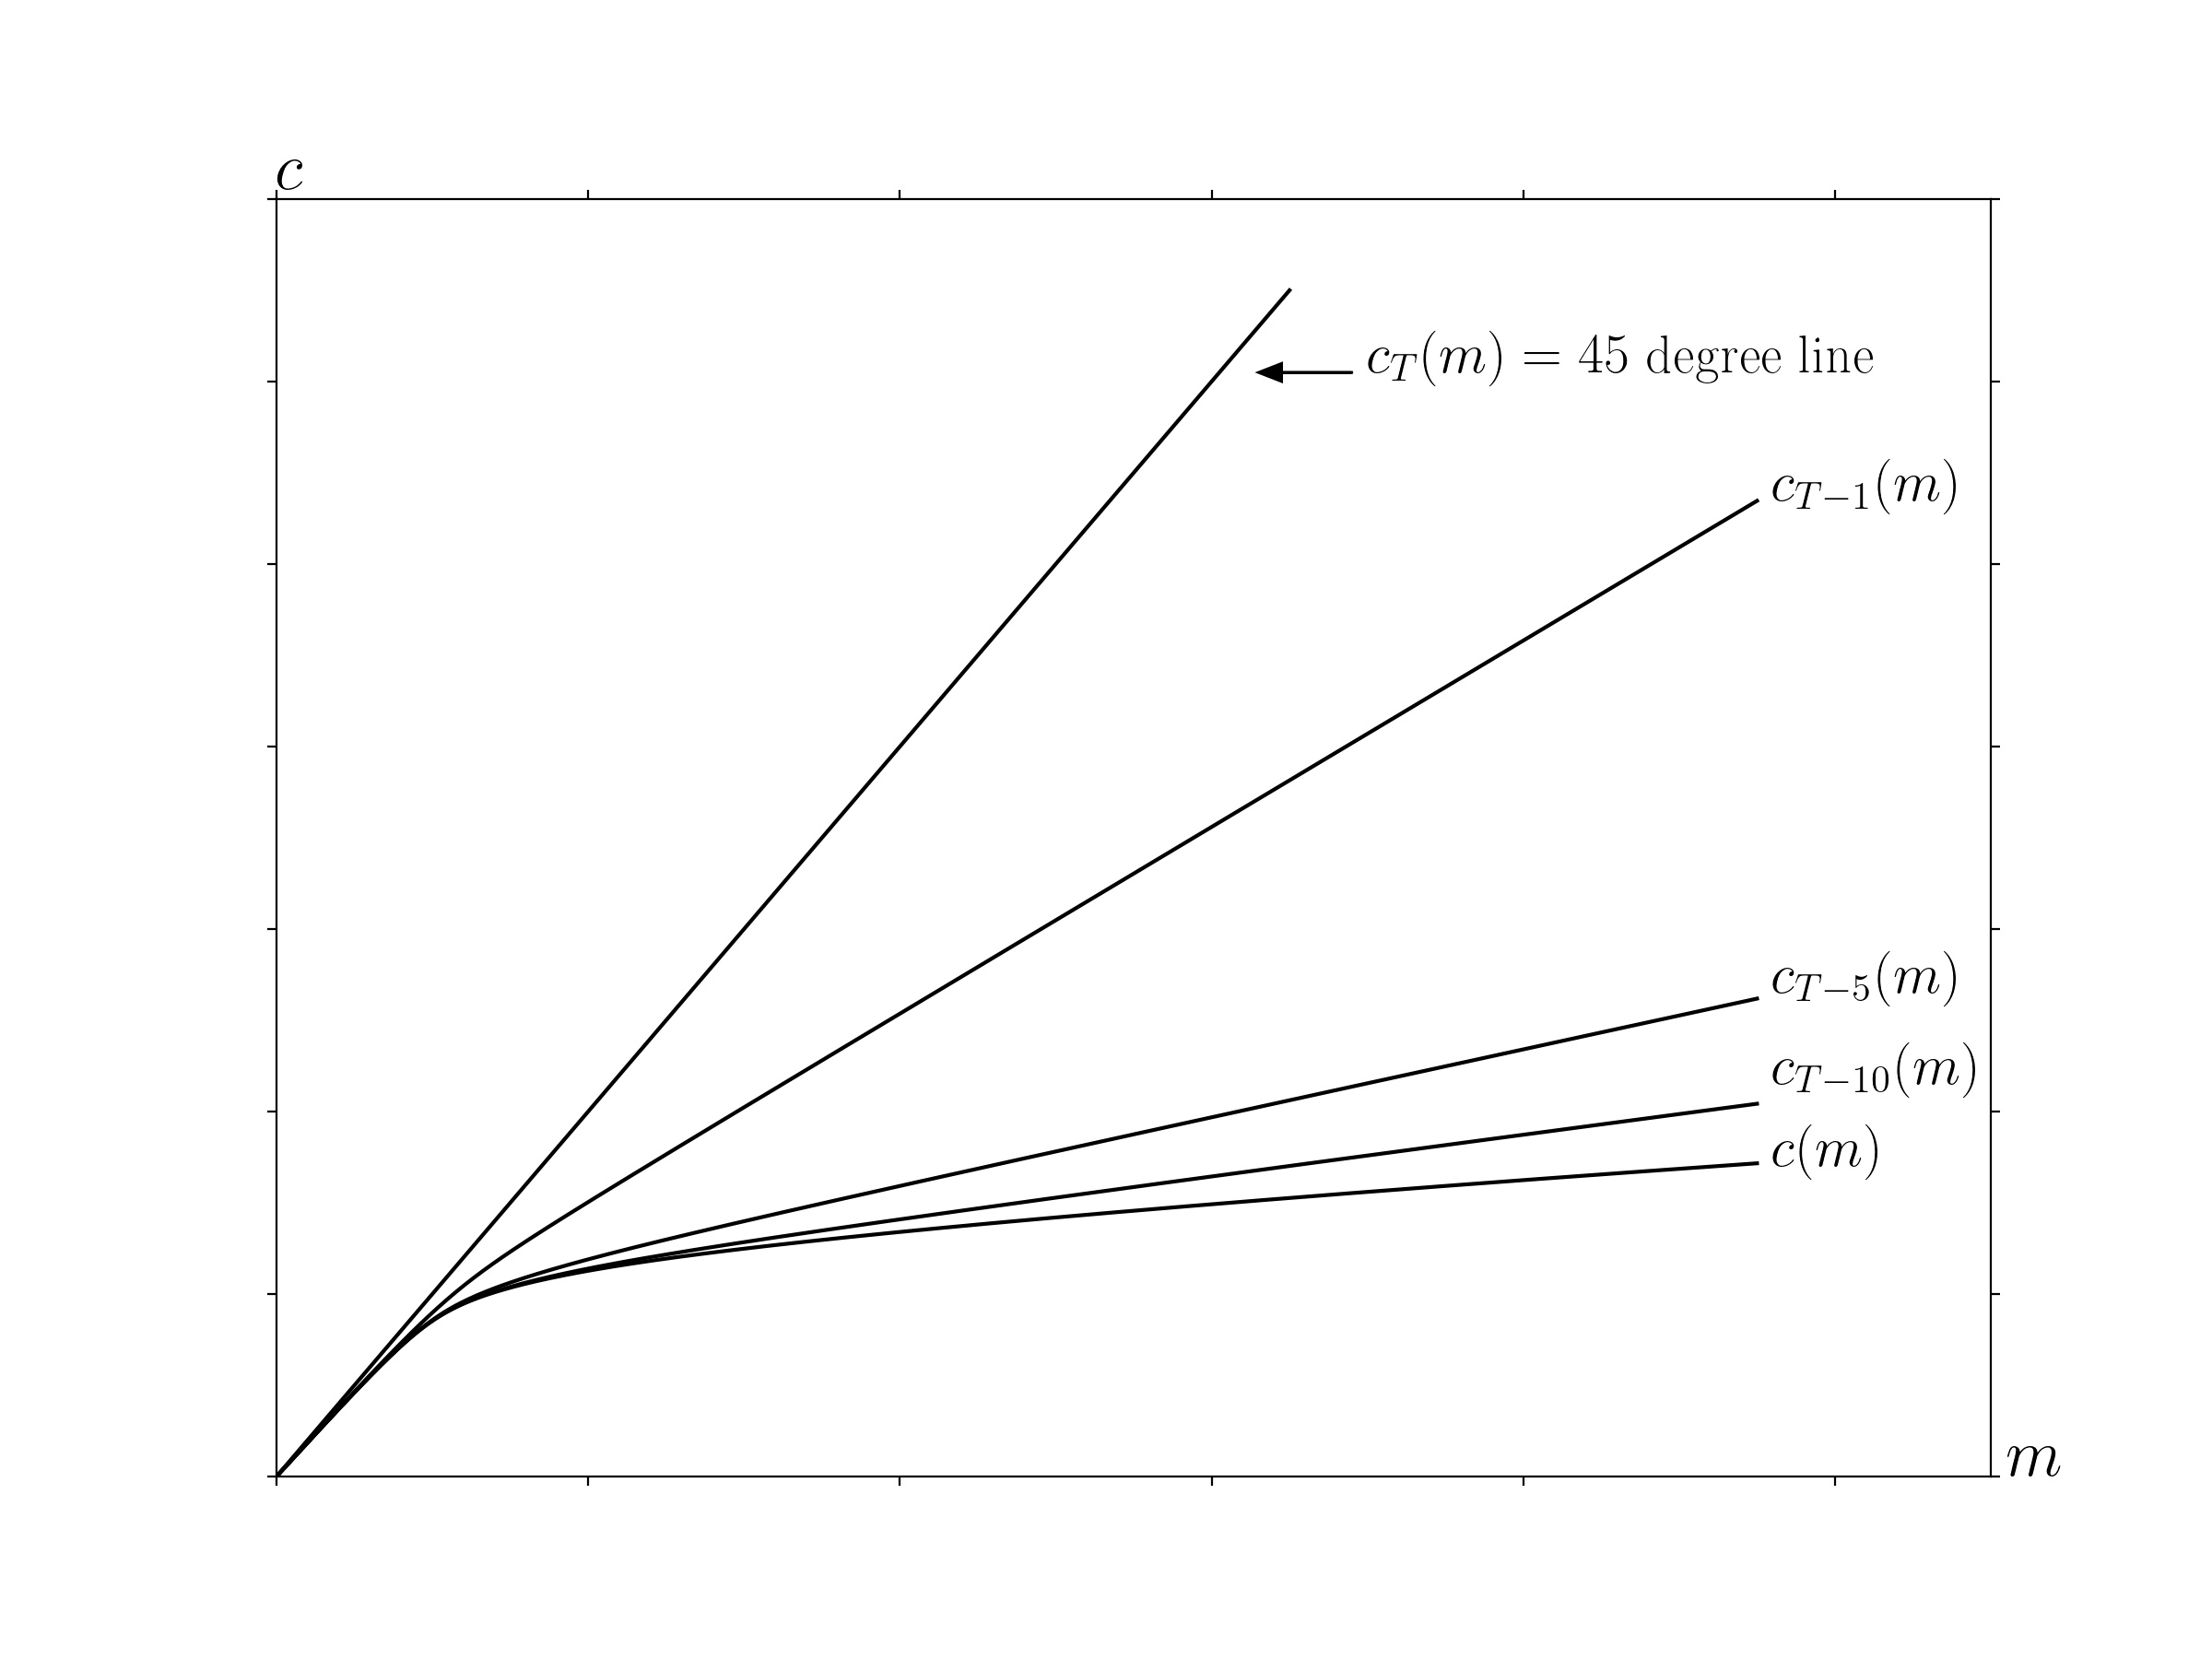
\includegraphics[width=5in]{\FigDir/cFuncsConverge}}
\caption{Convergence of the Consumption Rules}
\label{fig:cFuncsConverge}
\end{figure}
 % Read in the tex to generate the figure

In the figure, the consumption rules appear to converge as the horizon
recedes.  Our next purpose is to show that this appearance is not deceptive; we
call the hypothesized limiting infinite-horizon consumption rule
\begin{align}
  \cFunc(\mRat)  & \equiv  \lim_{n \rightarrow \infty} \cFunc_{T-n}(\mRat).
\end{align}

\hypertarget{Concave-Consumption-Function-Characteristics}{}
\subsection{Concave Consumption Function Characteristics}\label{sec:cExists}

A precondition for the main proof is that the maximization problem \eqref{eq:veqn} defines a sequence of continuously differentiable strictly increasing strictly concave\footnote{There is one obvious exception: $\cFunc_{T}(m)$ is a linear (and so only weakly concave) function.} functions $\{\cFunc_{T},\cFunc_{T-1},...\}$.\footnote{\cite{ckConcavity} proved concavity but not the other desired properties.}  The straightforward but tedious proof is relegated to appendix~\ref{sec:ApndxcExists}.  For present purposes, the most important point is the following intuition: $\cFunc_{t}(\mRat) < m$ for all periods $t < T$ because a consumer who spent all available resources would arrive in period $t+1$ with balances $b_{t+1}$ of zero, and then might earn zero noncapital income over the remaining horizon (an unbroken series of zero-income events is unlikely but possible).  In such a case, the budget constraint and the can't-die-in-debt condition mean that the consumer would be forced to spend zero, incurring negative infinite utility.  To avoid this disaster, the consumer never spends everything.  (This is an example of the `natural borrowing constraint' induced by a precautionary motive, per \cite{zeldesStochastic}).\footnote{It would perhaps be better to call it the `utility-induced borrowing constraint' as it follows from the assumptions on the utility function (in particular, $\lim_{c \downarrow 0} \uFunc(c)=-\infty$); for example, no such constraint arises if utility is of the (implausible) Constant Absolute Risk Aversion form.}

\hypertarget{Bounds-for-the-Consumption-Functions}{}
\subsection{Bounds for the Consumption Functions}

The consumption functions depicted in Figure~\ref{fig:cFuncsConverge} appear
to have limiting slopes as $\mRat \downarrow 0$ and as $\mRat \uparrow
\infty$.  This section confirms that impression and derives those
slopes, which also turn out to be useful in the contraction
mapping proof.\footnote{\cite{benhabibWealth} show that the consumption function
  becomes linear as wealth approaches infinity in a model with capital income risk and liquidity
  constraints; their results should generalize to the limits derived here if capital income risk were added to the model.}$^{,}$\footnote{\cite{MaStachurskiToda2020JET} establish the existence and uniqueness of a solution to a general income fluctuation problem with capital income risk in a Markovian setting and use such a model to study the tail behavior of wealth in the presence of risky returns to capital.}

\newcommand{\NewMaxMinMPC}{\ushort{\MPC}}

Assume (as discussed above) that a continuously differentiable
concave consumption function exists in period $t+1$, with an origin at
$\cFunc_{t+1}(0)=0$, a minimal MPC $\NewMaxMinMPC_{t+1}>0$, and
maximal MPC $\MaxMPC_{t+1} \leq 1$.  (If $t+1 = T$ these will be
$\NewMaxMinMPC_{T}=\MaxMPC_{T}=1$; for earlier periods they will exist
by recursion from the following arguments.)

The MPC bound as wealth approaches infinity is easy to understand: In this case,
under our imposed assumption that human wealth is finite, the proportion of consumption
that will be financed out of human wealth approaches zero. The
consequence is that the proportional difference between the solution to the
model with uncertainty and the perfect foresight model shrinks to zero.

\hypertarget{MPCnvrsLower}{}
\hypertarget{WRICCond}{}
In the course of proving this, appendix~\ref{sec:MPCLimits} provides a useful recursive expression for the (inverse of the) limiting MPC: 
\begin{align}
  \MinMPC_{t}^{-1}  & = 1+\MaxMPS \MinMPC_{t+1}^{-1} \label{eq:MinMPCInv}.
\end{align}

\subsubsection{Weak RIC Conditions}{}\label{sec:WRIC}
\hypertarget{MPCnvrsUpper}{}
\hypertarget{WRIC}{}
There is a parallel expression for the limiting maximal 
MPC as $\mRat \downarrow 0$: appendix equation \eqref{eq:MaxMPCInvApndx}  shows that, as $\mRat_{t} \uparrow \infty$,
\begin{align}
  \MaxMPC_{t}^{-1}  & = 1+\MinMPS \MaxMPC_{t+1}^{-1} \label{eq:MaxMPCInv}.
\end{align}
\hypertarget{WRIF}{}  
$\left\{\MaxMPC_{T-n}^{-1}\right\} _{n=0}^{\infty}$ is a decreasing % Correction per MNW 2016-01-30
convergent sequence if the `weak return patience factor' $\pZero^{1/\CRRA}\PatR$ satisfies:
\begin{align}
  0 \leq & \pZero^{1/\CRRA} \PatR < 1 \label{eq:WRIC},
\end{align}
a condition that we dub the `Weak Return Impatience Condition' (\WRIC)
because with $\pZero < 1$ it will hold more easily (for a larger set of parameter
values) than the \RIC~($\PatR < 1$).

The essence of the argument is that as wealth approaches zero, the overriding
consideration that limits consumption is the (recursive) fear of the zero-income events.  (That consideration is why the probability of the zero
income event $\pZero$ appears in the expression.)  

\hypertarget{cBounds}{}
We are now in position to observe that the optimal consumption function must satisfy
\begin{align}
  \MinMinMPC_{t} \mRat_{t} ~ \leq &   \cFunc_{t}(\mRat_{t})  \leq  ~ \MaxMPC_{t} \mRat_{t} \label{eq:cBounds}
\end{align}
because consumption starts at zero and is continuously differentiable (as argued above), is strictly concave (\cite{ckConcavity}), and always exhibits a slope between $\MinMinMPC_{t}$ and $\MaxMPC_{t}$ (the formal proof is provided in appendix \ref{sec:Tcomplete}).

These limits are useful at least in the sense that they can be hard-wired into a solution algorithm for the model, which has the potential to make the solution more efficient (cf.\ \cite{cctwMoM}).  Alternatively, they can provide a useful check on the accuracy of a solution algorithm that does not impose them directly.

\begin{comment}
  If the \FHWC~does not hold, we make do with a less useful bound on the minimal MPC: It is
  weakly greater than zero, which follows from the logic in
  \ref{sec:cExists}; hence the `max' in \eqref{eq:MinMinMPCDef}.
\end{comment}

\hypertarget{Conditions-Under-Which-the-Problem-Defines-a-Contraction-Mapping}{}
\subsection{Conditions Under Which the Problem Defines a Contraction Mapping}

\label{subsec:contraction}

To prove that the consumption rules converge, we need to show that the
problem defines a contraction mapping. This cannot be proven using the
standard theorems in, say, Stokey et.\ al.~\citeyearpar{slpMethods},
which require marginal utility to be bounded over the space of
possible values of $\mRat$, because the possibility (however unlikely)
of an unbroken string of zero-income events for the remainder of life
means that as $\mRat$ approaches zero $c$ must approach zero (see the
discussion in \ref{sec:cExists}); thus, marginal utility is unbounded.
Although a recent literature examines the existence and uniqueness 
of solutions to Bellman equations in the presence of `unbounded returns' (see, e.g.,
\cite{mnUnique}), the techniques in that literature
cannot be used to solve the problem here because the required conditions 
are violated by a problem that involves permanent shocks.\footnote{See \cite{yaoNote}
  for a detailed discussion of the reasons the existing literature up through \cite{mnUnique} cannot handle 
  the problem described here.}

Fortunately, Boyd~\citeyearpar{jboydWeighted} provided a weighted contraction mapping theorem that \cite{asHomogeneous} showed could be used to address the homogeneous case (of which CRRA formulation is an example) in a deterministic framework; later, \cite{duranDiscounting} showed how to extend the \cite{jboydWeighted} approach to the stochastic case.
\begin{defn}
  Consider any function $\bullet\in \mathcal{C}(\mathscr{A},\mathscr{B})$ where $\mathcal{C}(\mathscr{A},\mathscr{B})$ is the space of continuous functions from $\mathscr{A}$ to $%
  \mathscr{B}$. Suppose $\phiFunc \in \mathcal{C}(\mathscr{A},\mathscr{B})$ with $%
  \mathscr{B}\subseteq\mathbb{R}$ and $\phiFunc >0$. Then $\bullet$ is $\phiFunc$-bounded if the $\phiFunc$-norm of $\bullet$,
  \begin{equation}
    \Vert \bullet\Vert _{\phiFunc }=\sup_{\mRat}\left[ \frac{|\bullet(\mRat)|}{\phiFunc (\mRat)}\right] ,
    \label{eq:phinorm}
  \end{equation}%
  is finite.
\end{defn}

For $\mathcal{C}_{\phiFunc }\left( \mathscr{A},\mathscr{B}\right) $
defined as the set of functions in
$\mathcal{C}(\mathscr{A},\mathscr{B})$ that are $\phiFunc$-bounded;
$\wFunc$, $\xFunc$, $\yFunc$, and $\zFunc$ as examples of
$\phiFunc$-bounded functions; and using {$\mathbf{0}(\mRat)=0$} to
indicate the function that returns zero for any argument,
Boyd~\citeyearpar{jboydWeighted} proves the following.

\textbf{Boyd's Weighted Contraction Mapping Theorem.} \textit{Let $\BoydT:\mathcal{C}_{\phiFunc }\left( \mathscr{A},\mathscr{B}\right)
  \rightarrow \mathcal{C}\left( \mathscr{A},\mathscr{B}\right) $ such
  that}\footnote{We will usually denote the function that results from the mapping as, e.g., $\{\BoydT\wFunc\}$.}$^,$\footnote{To non-theorists, this notation may be slightly confusing; the inequality relations in (1) and (3) are taken to mean `for any specific element $\bullet$ in the domain of the functions in question' so that, e.g., $\xFunc \leq \yFunc$ is short for $\xFunc(\bullet) \leq \yFunc(\bullet)~\forall~\bullet\in \mathscr{A}.$  In this notation, $\zeta \Shrinker \phiFunc$ in (3) is a {\it function} which can be applied to any argument $\bullet$ (because $\phiFunc$ is a function).} \nopagebreak
\begin{align*}
  \mbox{(1)} &\BoydT%
               \mbox{ {\it is non-decreasing, i.e.\ ${\xFunc} \leq {\yFunc}\Rightarrow
               \{\BoydT{\xFunc}\} \leq \{\BoydT{\yFunc}\}$}}   \nonumber \\
  \mbox{(2)} & \{\BoydT\mathbf{0}\}\in ~ \mathcal{C}_{\phiFunc }\left(\mathscr{A},\mathscr{B}\right)  \notag \\
  \mbox{(3)}
             & \mbox{\it There exists some real $0 < \Shrinker < 1$, such that} \\
             & \{\BoydT({\wFunc} +\zeta\phiFunc )\} \leq \{\BoydT{\wFunc}\} +\zeta\Shrinker \phiFunc
               \mbox{ {\it ~holds for all real $\zeta > 0$} }.
\end{align*}%
\textit{Then $\BoydT$ defines a contraction with a unique fixed point.}

For our problem, take $\mathscr{A}$ as $\mathbb{R}_{>0}$ and $\mathscr{B}$
as $\mathbb{R}$, and define
\begin{align*}
  \{\EEndMap \zFunc\}(a_{t})  & = \Ex_{t}\left[\PGro^{1-\CRRA}_{t+1} \zFunc(a_{t} \Rnorm_{t+1} + \tShkAll_{t+1})\right].
\end{align*}

Using this, we introduce the mapping \textit{$\TMap:\mathcal{C}_{\phiFunc }\left( \mathscr{A},\mathscr{B}\right) \rightarrow \mathcal{C}\left(
    \mathscr{A},\mathscr{B}\right) $},\footnote{Note that the existence of the maximum is assured by the continuity of $\{\EEndMap \zFunc\}(a_{t})$ (it is continuous because it is the sum of continuous $\phiFunc$-bounded functions $\zFunc$) and the compactness of $[\MinMinMPC \mRat_{t},  \MaxMPC \mRat_{t}]$.}
\begin{comment} %
  (In the subtle case when $\MinMinMPC=0$, the compact interval could be revised as $ [(\MinMinMPC+\epsilon) \mRat_{t},
  \MaxMPC \mRat_{t}]$ where $\epsilon$ is a very small positive number because obviously $\MinMinMPC \mRat_{t}=0$ will not be the $\argmax$)
\end{comment}
\begin{align}
  \{\TMap{\zFunc}\}(\mRat_{t})  & = \underset{{\cRat}_{t} \in
                                  [\MinMinMPC \mRat_{t}, \MaxMPC \mRat_{t}]
                                  } \max
                                  \uFunc(c_{t})+\DiscFac \left( \{\EEndMap \zFunc \}(\mRat_{t}-c_{t}) \right)  \label{definitionmappingT}.
\end{align}

\begin{comment}
  Unpacking the definitions, our mapping $\TMap$ can be written more explicitly as
  \begin{align}
    \{\TMap\zFunc\}(\mRat_{t})  & = \underset{\cRat_{t} \in [\MinMinMPC
                                  \mRat_{t}, \MaxMPC \mRat_{t}]} \max \left\{
                                  \uFunc(c_{t})+\DiscFac \Ex_{t}\left[ {\PGro}_{t+1} ^{1-\CRRA }\zFunc(
                                  {\aRat}_{t}\Rnorm_{t+1}+\tShkAll_{t+1}) \right] \right\}
                                  .
  \end{align}
\end{comment}

\hypertarget{Contraction-Conditions}{}

We can show that our operator $\TMap$ satisfies the conditions that
Boyd requires of his operator $\BoydT$, if we impose two restrictions
on parameter values.  The first is the \WRIC~necessary for
convergence of the maximal MPC, equation \eqref{eq:WRIC} above.  A
more serious restriction is the utility-compensated Finite Value of
Autarky condition, equation \eqref{eq:FVAC}.  (We discuss the
interpretation of these restrictions in detail in section
\ref{sec:discussConvergence} below.)  Imposing these restrictions, we
are now in position to state the central theorem of the paper.

\hypertarget{MainTheorem}{}
\setcounter{theorem}{0}
\begin{theorem}
  \label{thm:contmap} $\TMap$ is a contraction mapping if
  the restrictions on parameter values \eqref{eq:WRIC} and
  \eqref{eq:FVAC} are true (that is, if the weak return impatience condition and the finite value of autarky condition hold).
\end{theorem}

Intuitively, Boyd's theorem shows that if you can find a $\phiFunc$ that is everywhere finite but goes to infinity `as fast or faster' than the function you are normalizing with $\phiFunc$, the normalized problem defines a contraction mapping.  The intuition for the {\FVAC} condition is just that, with an infinite horizon, with any initial amount of bank balances $\bRat_{0}$, in the limit your value can always be made greater than you would get by consuming exactly your permanent income every period (say, by consuming $(\rfree/\Rfree)\bRat_{0}-\epsilon$ for some small $\epsilon>0$).

The details of the proof are cumbersome, and are therefore relegated to
appendix~\ref{sec:Tcomplete}.  Given that the value function
converges, appendix~\ref{subsec:cConverges} shows that the consumption
functions converge.

\hypertarget{The-Liquidity-Constrained-Solution-as-a-Limit}{}
\subsection{The Liquidity Constrained Solution as a Limit} \label{sec:deatonIsLimit}

This section shows that a related problem commonly considered in the
literature (e.g., with a simpler income process, by
Deaton~\citeyearpar{deatonLiqConstr}), with a liquidity constraint
and a positive minimum value of income, is the limit of the problem
considered here as the probability $\pZero$ of the zero-income event
approaches zero.

The essence of the argument is easy to state.  As noted above, the possibility of earning zero income over the remainder of the horizon prevents the consumer from ending the current period with zero assets because with some finite probability the consumer would be forced to consume zero, which would be infinitely painful.

But the \textit{extent} to which the consumer feels the need to make this
precautionary provision depends on the probability that it will turn
out to matter.  As $\pZero \downarrow 0$, that probability becomes
arbitrarily small, so the amount of precautionary saving approaches zero.
But zero precautionary saving is the amount of saving that a liquidity
constrained consumer with perfect foresight would choose.

Another way to understand this is just to think of the liquidity
constraint as being imposed by specifying a component of the utility
function that is zero whenever the consumer ends the period with
(strictly) positive assets, but negative infinity if the consumer
ended the period with (weakly) negative assets.

See appendix \ref{sec:LiqConstrAsLimit} for the formal proof justifying the
foregoing intuitive discussion.

\hypertarget{Discussion-of-Parametric-Restrictions}{}
\subsection{Discussion of Parametric Restrictions}\label{sec:discussConvergence}

The full relationship among all the conditions articulated above is represented in Figure~\ref{fig:Inequalities}.
Though the diagram looks complex, it is merely a modified version of the earlier diagram with further 
(mostly intermediate) inequalities inserted.  Again readers unfamiliar with such diagrams should Appendix~\ref{sec:ApndxConditionDiagrams}) for a more detailed explanation.

\renewcommand{\figName}{Inequalities} % Allows generic definition of hypertargets based on title of figure
\renewcommand{\figFile}{\figName} %  and on filename
\hypertarget{\figFile}{}
\hypertarget{\figName}{}
\input{\FigDir/\figName} % Read in the tex to generate the figure

\begin{comment}
  \subsubsection{Perfect Foresight Case}

  The unconstrained perfect foresight model is the natural starting
  point for developing the intuition behind our parametric restrictions.
  As noted above, the Return Impatience Condition (\RIC) is necessary in
  this context to guarantee that the PDV of the stream of future
  consumption is finite; value is then given by
  \begin{align*}
    \vLevBF_{t}  & = \uFunc(\cLevBF_{t})+\DiscFac \uFunc(\overbrace{(\Rfree \DiscFac)^{1/\CRRA}\cLevBF_{t}}^{=\cLevBF_{t+1}})+\DiscFac^{2} \uFunc(((\Rfree \DiscFac)^{1/\CRRA})^{2}\cLevBF_{t})+...
    \\  & = \uFunc(\cLevBF_{t})\left(1+\DiscFac ((\Rfree \DiscFac)^{1/\CRRA})^{1-\CRRA}+(\DiscFac ((\Rfree \DiscFac)^{1/\CRRA})^{1-\CRRA})^{2}+...\right)
  \end{align*}
  which has a finite limit so long as $\DiscFac ((\Rfree \DiscFac)^{1/\CRRA})^{1-\CRRA} < 1$.  But
  \begin{align*}
    \DiscFac ({\Pat})^{1-\CRRA}   & = \DiscFac (\DiscFac \Rfree)^{1/\CRRA - 1}
    \\  & = {\Pat}/\Rfree = \PatR
  \end{align*}
  so the \RIC~guarantees the finiteness of value in addition to the PDV
  of consumption (given a finite starting point).

  The starting point for consumption is guaranteed to be finite by
  imposition of the finite human wealth (\FHWC) requirement.  (If human
  wealth were unbounded, our unconstrained consumer could freely borrow
  in order to spend an infinite amount in every period.)

  An alternative way to limit consumption is by imposing a liquidity
  constraint $\cRat_{t} \leq \mRat_{t}$.  Naturally, in the presence of
  such an urgent constraint, other constraints become less important.
  Indeed, the strength of the liquidity constraint can be appreciated
  from the fact that it prevents consumption from exceeding current
  resources even when human wealth is infinite.

  Value, in the constrained case, is easy to calculate, because the
  constrained consumer's spending is always equal to income, which
  always grows by $\PGro$:
  \begin{align}
    \vLevBF_{t}  & = \uFunc(\pLevBF_{t})+\DiscFac \uFunc(\pLevBF_{t} \PGro) + \DiscFac^{2} \uFunc(\pLevBF_{t} \PGro^{2}) ... \notag
    \\  & = \uFunc(\pLevBF_{t})\left(1+\DiscFac \PGro^{1-\CRRA}+(\DiscFac \PGro^{1-\CRRA})^{2}+...\right)
  \end{align}
  which explains the perfect foresight finite value requirement
  \eqref{eq:FVAC}: It guarantees that value for the constrained
  consumer is finite.  Thus, the introduction of constraints is what
  makes the finite value requirement interesting; with finite value it becomes
  possible to calculate the consequences of alternatives.
\end{comment}

\hypertarget{IntuitionRIC}{}
\subsubsection{The \RIC}

In the perfect foresight unconstrained problem
(section~\ref{subsec:PFUncon}), the \RIC~was required for existence of
a nondegenerate solution.  It is surprising, therefore, that in the
presence of uncertainty, the \RIC~is neither necessary nor sufficient
for a nondegenerate solution.
\begin{comment}
  But if the \RIC~does hold, some useful results can be derived.  Arguably
  the most fundamental are that the limiting values
  for the minimal and maximal marginal propensities to consume implicit in
  \eqref{eq:MaxMPCInv} and \eqref{eq:MinMPCInv} are positive and finite.
\end{comment}
We thus begin our discussion by asking what features the problem must
exhibit (given the \FVAC) if the \RIC~fails (that is, $\Rfree < (\Rfree \DiscFac)^{1/\CRRA})$:
\begin{align}
  \Rfree   & < \overbrace{(\Rfree \DiscFac)^{1/\CRRA} ~ < ~ (\Rfree (\PGro \uInvEpShkuInv)^{\CRRA-1})^{1/\CRRA}}^{\text{implied by \FVAC}} \notag
  \\  \Rfree   & < (\Rfree/\PGro)^{1/\CRRA}\PGro \uInvEpShkuInv^{1-1/\CRRA} \notag
  \\  \Rfree/\PGro  & < (\Rfree/\PGro)^{1/\CRRA}\uInvEpShkuInv^{1-1/\CRRA} \notag
  \\  (\Rfree/\PGro)^{1-1/\CRRA}  & < \uInvEpShkuInv^{1-1/\CRRA} \label{eq:RICimplies}
\end{align}
but since $\uInvEpShkuInv<1$ and $0 < 1-1/\CRRA < 1$ (because we have
assumed $\CRRA > 1$), equation \eqref{eq:RICimplies} this can hold only if $\Rfree/\PGro < 1$; that
is, given the \FVAC, the \RIC~can fail only if human wealth is
unbounded.  Unbounded human wealth is permitted here, as in the
perfect foresight liquidity constrained problem.  But,
from  equation
\eqref{eq:MinMPCInv}, an implication of \cncl{\RIC} is that $\lim_{m
  \uparrow \infty} \cFunc^{\prime}(m) = 0$.  Thus, interestingly,
the presence of uncertainty both permits unlimited human wealth and at
the same time prevents that unlimited wealth from resulting in
infinite consumption.  That is, in the presence of uncertainty,
pathological patience (which in the perfect foresight model with
finite wealth results in consumption of zero) plus infinite human
wealth (which the perfect foresight model rules out because it leads
to infinite consumption) combine here to yield a unique finite
limiting MPC for any finite value of $\mRat$.  Note
the close parallel to the conclusion in the perfect foresight
liquidity constrained model in the
\{\PFGIC,\cncl{\RIC}\} case (for detailed analysis of this
case see appendix \ref{sec:ApndxLiqConstr}).  There, too, the tension between infinite human wealth
and pathological patience was resolved with a nondegenerate consumption function
whose limiting MPC was zero.

\subsubsection{The \WRIC}

The `weakness' of the additional requirement for contraction, the
weak \RIC, can be seen by asking `under what circumstances
would the \FVAC~hold but the \WRIC~fail?'
Algebraically, the requirement is
\begin{align}
  \DiscFac \PGro^{1-\CRRA}\uInvEpShkuInv^{1-\CRRA} & < ~ 1 ~ <  (\pZero \DiscFac)^{1/\CRRA}/\Rfree^{1-1/\CRRA}. \label{eq:WRICandFVAC}
\end{align}

If there were no conceivable parameter values that could satisfy both
of these inequalities, the \WRIC~would have no force.  And if we require $\Rfree \geq 1$, the \WRIC~is indeed
redundant because now $\DiscFac <1<\Rfree^{\CRRA-1}$, so that the \RIC~(and \WRIC) must hold.

But neither theory nor evidence demands that we assume $\Rfree \geq
1$.  We can therefore approach the question of the \WRIC's relevance by
asking just how low $\Rfree$ must be for the condition to be relevant.
Suppose for illustration that $\CRRA=2$, $\uInvEpShkuInv^{1-\CRRA}=1.01$,
$\PGro^{1-\CRRA}=1.01^{-1}$ and $\pZero = 0.10$.  In that case
\eqref{eq:WRICandFVAC} reduces to
\begin{align}
  \DiscFac  & < 1 < (0.1 \DiscFac/\Rfree)^{1/2} \notag
\end{align}
but since $\DiscFac < 1$ by assumption, the binding requirement is that
\begin{align}
  \Rfree  & < \DiscFac/10 \notag
\end{align}
so that for example if $\DiscFac=0.96$ we would need $\Rfree < 0.096$
(that is, a perpetual riskfree rate of return of worse than -90
percent a year) in order for the \WRIC~to bind.
The relevance of the \WRIC~is indeed ``Weak.''

Perhaps the best way of thinking about this is to note that the space
of parameter values for which the \WRIC~is relevant shrinks out of
existence as $\pZero \rightarrow 0$, which section
\ref{sec:deatonIsLimit} showed was the precise limiting condition
under which behavior becomes arbitrarily close to the liquidity
constrained solution (in the absence of other risks).  On the other
hand, when $\pZero = 1$, the consumer has no noncapital income (so
that the \FHWC~holds) and with $\pZero=1$ the \WRIC~is identical to the
RIC; but the \RIC~is
the only condition required for a solution to exist
for a perfect foresight consumer with no noncapital income.  Thus the
WRIC~forms a sort of `bridge' between the liquidity constrained and
the unconstrained problems as $\pZero$ moves from 0 to 1.

\hypertarget{The-GIC}{}
\hypertarget{When-the-GIC-Fails}{}
\subsubsection{When the \GIC~Fails}\label{sec:WhenTheGICFails}

If both the \GIC~and the \RIC~hold, the arguments above establish that the limiting consumption
function asymptotes to the consumption function for the perfect foresight unconstrained function.
The more interesting case is where the \GIC~fails.
\begin{comment}
  \WW{}{The same
    steps as above lead to the same implication that this requires
    $\InvEpShkInv < (\Rfree/\PGro)^{1/\CRRA}\uInvEpShkuInv^{1-1/\CRRA}$,
    but when the \RIC~$\Rfree/\PGro > 1$ holds this condition is much more
    easily satisfied.}
  If the \FVAC~holds but the \GIC~does not, the parameters must satisfy:
  \begin{align}
    \DiscFac \PGro^{1-\CRRA}\Ex[\pshk^{1-\CRRA}] & < 1 < (\Rfree\DiscFac)^{1/\CRRA}(\PGro\Ex[\pshk^{-1}])^{-1}. \label{eq:FVACnotGIC}
  \end{align}

  Note first that by Jensens's inequality $\Ex[\pshk^{1-\CRRA}] > 1$ and $(\Ex[\pshk^{-1}])^{-1} < 1$,
  so \eqref{eq:FVACnotGIC} is stronger than
  \begin{align}
    \DiscFac \PGro^{1-\CRRA} & < 1 < (\Rfree\DiscFac)^{1/\CRRA}/\PGro. \label{eq:PFFVACnotPFGIC}
  \end{align}

  Suppose $\PGro=1$, $\CRRA=2$ and $\pshk$ is lognormally distributed with $\sigma^{2}_{\pshk}=0.01$ (that is, $\log \pshk \sim \mathcal{N}(-\sigma_{\psi}^{2}/2,\sigma_{\psi}^{2})$) so that $\Ex_{t}[\pshk_{t+1}^{1-\CRRA}] =\Ex_{t}[\pshk_{t+1}^{-1}] =\exp(\sigma^{2}_{\psi})=e^{0.01}.$  Then the condition becomes
  \begin{align}
    \DiscFac e^{0.01} & < 1 < (\Rfree \DiscFac)^{1/2}e^{-0.01}
  \end{align}
  which can be satisfied, for example, by $\DiscFac = 0.96$ and $\Rfree=1.08$.
\end{comment}
A solution that satisfies the combination \FVAC~and
\cncl{\GIC} is depicted in Figure \ref{fig:FVACnotGIC}.  The
consumption function is shown along with the $\Ex_{t}[\Delta
\mRat_{t+1}]=0$ locus that identifies the `sustainable' level of
spending at which $\mRat$ is expected to remain unchanged.  The
diagram suggests a fact that is confirmed by deeper analysis: Under
the depicted configuration of parameter values (see the code for details), the consumption function never reaches the
$\Ex_{t}[\Delta \mRat_{t+1}]=0$ locus; indeed, when the \RIC~holds but
the \GIC~does not, the consumption function's limiting slope
$(1-\Pat/\Rfree)$ is shallower than that of the sustainable consumption
locus $(1-\PGroAdj/\Rfree)$,\footnote{This is because
  $\Ex_{t}[\mRat_{t+1}]=\Ex_{t}[\Rnorm_{t+1}(\mRat_{t}-\cRat_{t})]+1$; solve $\mRat = (\mRat - \cRat)\Rnorm \InvEpShkInv^{-1}+1$ for $\cRat$ and differentiate.}
so the gap between the two actually increases with $\mRat$ in the
limit.  Although a nondegenerate consumption function
exists, a target level of $\mRat$ does not (or, rather, the
target is $\mRat=\infty$), because no matter how wealthy a consumer
becomes, the consumer will always spend less than the amount that
would keep $\mRat$ stable (in expectation).

\renewcommand{\figFile}{FVACnotGIC}
\hypertarget{\figFile}{}
\hypertarget{FVACnotGIC}{}
\begin{figure}[tbp]
\centerline{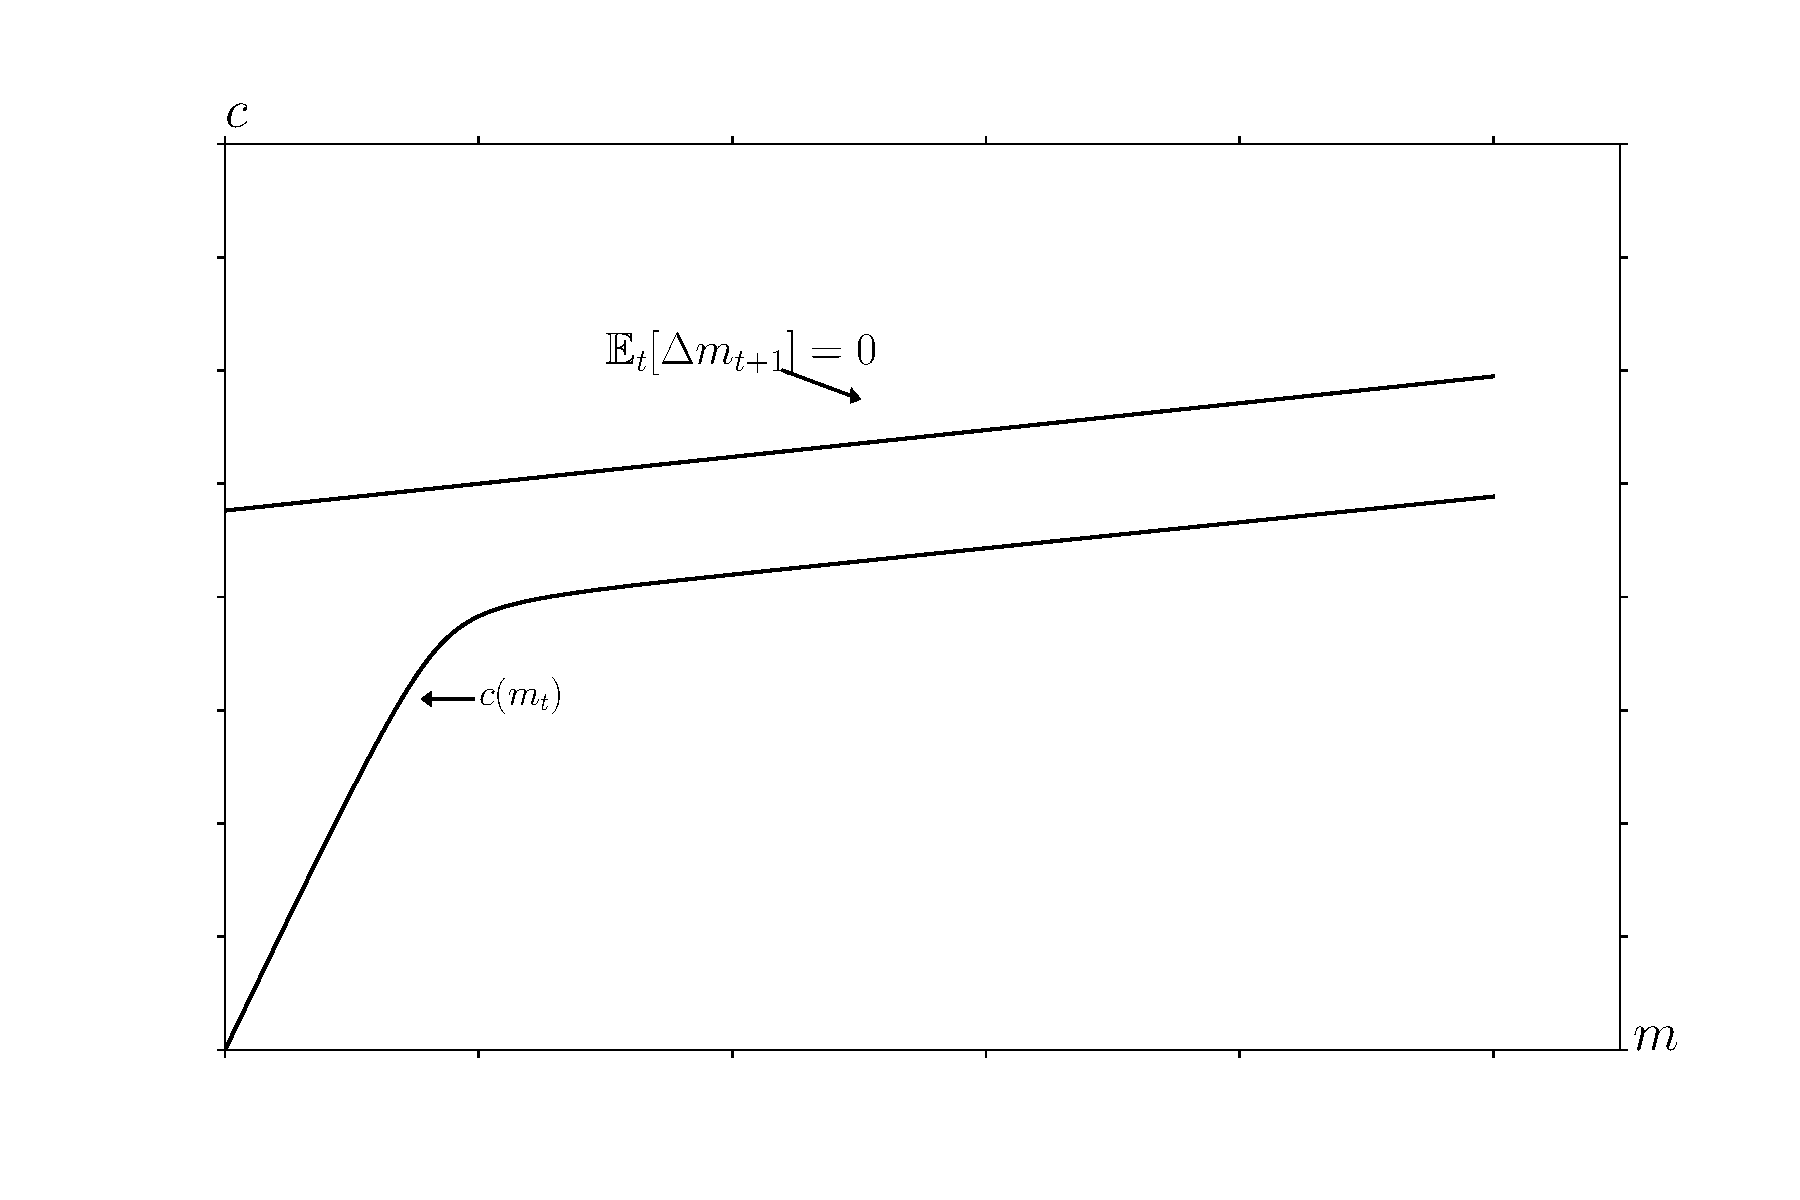
\includegraphics[width=6in]{\FigDir/FVACnotGIC}}
\caption{Example Solution when \FVAC~Holds but \GIC~Does Not}
\label{fig:FVACnotGIC}
\end{figure}


\begin{comment}
  The foregoing has some connection with the theoretical results in
  Szeidl~\citeyearpar{szeidlInvariant}, who shows that the condition we
  call the \GIC~guarantees that $\mRat$ will have an asymptotically
  bounded mean.  He also shows that under these circumstances $\mRat$
  satisfies conditions he proves to be necessary for the existence of a
  stable invariant distribution.  Furthermore, $\aRat$, $\bRat$, and $\cRat$
  are also shown to have stable invariant distributions and asymptotically
  bounded means.  We make use of these results below.
\end{comment}

\begin{comment} % Not really necessary
  A final point worth reemphasizing is that neither the Return
  Impatience Condition nor the Finite Human Wealth Condition was
  required for the contraction mapping proof.  Both these conditions are
  necessary for a nondegenerate solution to exist in the unconstrained
  perfect foresight case.  This is noteworthy because in some models and
  in many economists' intuition, the introduction of uncertainty reduces
  the space of parameter values for which a unique solution exists;
  here, precisely the opposite occurs.  Indeed, many of the
  parameterizations newly eligible for solution are quite plausible, so
  this observation is not merely a curiosum but of real practical
  value.\footnote{An easy example of a case where the perfect foresight
    model has no solution is where $\Rfree >1$, $\DiscFac = 1/\Rfree$
    and $\PGro > \Rfree$.}
\end{comment}

Tables \ref{table:Comparison} and \ref{table:Required} present a summary of the connections between the various conditions in the presence and the absence of uncertainty.

\hypertarget{Factors-Defined-And-Compared}{}
\subfile{\TableDir/Comparison-subfile}

\hypertarget{Sufficient-Conditions}{}
\hypertarget{Sufficient-Conditions-For-Nondegenerate-Solution}{}

\newsavebox{\Required}
\begin{table}
\centering
\caption{Sufficient Conditions for Nondegenerate$^{\ddagger}$ Solution} \label{table:Required}
\sbox{\Required}{
\begin{tabular}{|l|l|l|} \hline
%                                            & \multicolumn{1}{c|}{Required}   & \multicolumn{1}{c|}{}  \\
\multicolumn{1}{|c|}{Model}              & \multicolumn{1}{c|}{Conditions} & \multicolumn{1}{c|}{Comments/Logic}
\\ \hline
   \multicolumn{1}{|l|}{PF Unconstrained}   & \RIC, \FHWC$^{\circ}$                       & \RIC~$\Rightarrow |\vFunc(\mRat)|< \infty$; \FHWC~$\Rightarrow 0 < |\vFunc(\mRat)|$
\\ \href{https://\owner.github.io/BufferStockTheory\#PF-Constrained-Solution}{\phantom{~~}Section~\ref{subsec:PFUncon}}                                         &                                 & \RIC~prevents $\bar{\cFunc}(\mRat)=0$
\\                                          &                                 & \FHWC~prevents $\bar{\cFunc}(\mRat)=\infty$
%\\                                          &                                 & See \href{https://\owner.github.io/BufferStockTheory\#PF-Constrained-Solution}{Section~\ref{subsec:PFUncon}}
  \\ \hline\hline \multicolumn{1}{|l|}{PF Constrained}     & \cncl{\PFGIC}, \RIC & {\FHWC} must hold $(\PGro < \Pat < \Rfree \Rightarrow \PGro < \Rfree)$
                                                                                    \\ & & Identical to solution to PF Unconstrained for
% \\                               &                                  & See \href{https://\owner.github.io/BufferStockTheory\#PF-Constrained-Solution}{Section~\ref{subsec:PFCon}, Appendix~\ref{sec:ApndxLiqConstr}}
  \\                                                                 \href{https://\owner.github.io/BufferStockTheory\#PF-Constrained-Solution}{\phantom{~~}Section~\ref{subsec:PFCon}}                                                                         & & $  \mRat > \mRat_{\#}$ for some $0 < \mRat_{\#} < 1$; $\cFunc(\mRat)=\mRat$ for $\mRat \leq \mRat_{\#}$
\\ & & (\cncl{\RIC} would yield $\mRat_{\#}=0$ so degenerate $\cFunc(\mRat)=0$)
  \\ \cline{2-3} \href{https://\owner.github.io/BufferStockTheory\#ApndxLiqConstr}{\phantom{~~}Appendix~\ref{sec:ApndxLiqConstr}} & \PFGIC,\RIC & $\lim_{\mRat \rightarrow \infty} \mathring{\cRat}(\mRat)=\bar{\cRat}(\mRat), \lim_{\mRat \rightarrow \infty} \mathring{\MPCFunc}(\mRat)=\MinMPC$
\\                                          &                                 & kinks at points where horizon to $b=0$ changes$^{\ast}$
% \\                               &                                  & See \href{https://\owner.github.io/BufferStockTheory\#PF-Constrained-Solution}{\phantom{~~}Section~\ref{subsec:PFCon}, Appendix~\ref{sec:ApndxLiqConstr}}
  \\ \cline{2-3}                              &   \PFGIC,\cncl{\RIC}    & $\lim_{\mRat \rightarrow \infty} \mathring{\MPCFunc}(\mRat)=0$
\\                                          &                                 & kinks at points where horizon to $b=0$ changes$^{\ast}$
%\\                               &                                 & See \href{https://\owner.github.io/BufferStockTheory\#PF-Constrained-Solution}{Section~\ref{subsec:PFCon}, Appendix~\ref{sec:ApndxLiqConstr}}
\\ \hline\hline \multicolumn{1}{|l|}{Buffer Stock Model} & \FVAC, \WRIC~                     & \FHWC~$\Rightarrow$ $\lim_{\mRat \rightarrow \infty} \mathring{\cRat}(\mRat)=\bar{\cRat}(\mRat), \lim_{\mRat \rightarrow \infty} \mathring{\MPCFunc}(\mRat)=\MinMPC$
  \\ \href{https://\owner.github.io/BufferStockTheory\#Uncertainty-Modified-Conditions}{\phantom{~~}Section~\ref{subsec:UncertaintyModifiedConditions}}
                                            &                                 & \cncl{\FHWC}+RIC~$\Rightarrow \lim_{\mRat \rightarrow \infty} \mathring{\MPCFunc}(\mRat)=\MinMPC$
\\                                          &                                 & \cncl{\FHWC}+\cncl{\RIC} $\Rightarrow \lim_{\mRat \rightarrow \infty} \mathring{\MPCFunc}(\mRat)=0$
\\                                          &                                 & \GIC~guarantees finite target wealth ratio
\\                                          &                                 & \FVAC~is stronger than \PFFVAC~
\\                                          &                                 & \WRIC~is weaker than \RIC~
\\ \hline \multicolumn{3}{c}{}
\end{tabular}
} % End \sbox

\settowidth\TableWidth{\usebox{\Required}}
\usebox{\Required}

\parbox{\TableWidth}{\footnotesize         $^{\ddagger}$For feasible $\mRat$ satisfying $0 < \mRat < \infty$, a nondegenerate limiting consumption function defines the unique value of $\cRat$ satisfying $0 < \cRat(m) < \infty$; a nondegenerate limiting value function defines a corresponding unique value of $-\infty < \vFunc(\mRat) < 0$ .\phantom{~~}$^{\circ}$RIC, \FHWC~are necessary as well as sufficient.\phantom{~~}$^{\ast}$That is, the first kink point in $\cRat(\mRat)$ is $\mRat_{\#}$ s.t. for $\mRat < \mRat_{\#}$ the constraint will bind now, while for $\mRat > \mRat_{\#}$ the constraint will bind one period in the future.  The second kink point corresponds to the $\mRat$ where the constraint will bind two periods in the future, etc.} %\phantom{~~}$^{\ast}$Solution also exists for \cncl{\PFGIC} and \RIC, but is identical to the unconstrained model's solution for feasible $\mRat \geq 1$.
\end{table}



\begin{comment}
  To help interpret our condition, consider an infinite horizon perfect
  foresight consumer who does satisfy $\PGro < \Rfree$ and who arrives in period
  $t$ with beginning-of-period resources of zero, so that he has only
  human wealth.  If initial permanent income is $\pLevBF_{t}$ then
  $\hLevBF_{t}=\pLevBF_{t}(\Rfree/(\Rfree-\PGro))$ and the formula for consumption \eqref{eq:WDef} becomes
  \begin{align}
    \cLevBF_{t}  & = \left(\frac{\Rfree - {\Pat}}{\Rfree-\PGro}\right)\pLevBF_{t}
  \end{align}
  so the condition ${\Pat} < \PGro$ guarantees that consumption
  will exceed noncapital income of $\pLevBF_{t}$.  Thus, this consumer is `impatient'
  in the sense of wanting to borrow against future noncapital income to finance
  current consumption (this justifies our labeling of \eqref{eq:GIC} as the
  `growth impatience condition.')

  The presence of permanent shocks tightens the restriction, since if
  $\pShk$ is nondegenerate then $\Ex[\pShk^{-\CRRA}]^{-1/\CRRA} > 1$.  The
  interpretation of this effect is simple: The presence of uncertainty
  in permanent income increases the consumer's precautionary saving
  motive, and therefore increases the degree of patience; the condition
  requires that even after this boost to the saving motive, the consumer
  remains impatient in the relevant sense.

  The simplest intuition for why our model has a solution when $\PGro>\Rfree$
  comes from the essential equivalence between the precautionary saving
  motive and liquidity constraints. Consider a version of the perfect
  foresight model with liquidity constraints.  This model {\it does}
  have a well defined solution for $\PGro>\Rfree$ because even a consumer with
  considerable current resources cannot spend an infinite amount (even
  if the PDV of future noncapital income is infinite) because that would
  violate the constraint.  Furthermore, the amount the consumer is
  willing to spend today is limited by the knowledge that, because of
  impatience, they will be constrained at some point in the future.

  The precautionary motive induced by the noncapital income risk can be
  thought of as being like a smoothed version of liquidity constraints.
  As cash declines toward zero, the size of the risk relative to the
  size of cash increases, which means that the relative variation in
  consumption increases, which means that the intensity of the
  precautionary motive increases.  For a more rigorous and detailed
  treatment of the relationship between precautionary saving and
  liquidity constraints, see Carroll and
  Kimball~\citeyearpar{carroll&kimball:liquidity}.
\end{comment}

\hypertarget{AnalysisoftheConvergedConsumptionFunction}{}
\section{Analysis of the Converged Consumption Function}

Figures~\ref{fig:cGroTargetFig} and \ref{fig:mpclimits}a,b capture the
main properties of the converged consumption rule when the \RIC, \GIC,
and \FHWC~all hold.\footnote{These figures reflect the converged rule
  corresponding to the parameter values indicated in
  Table~\ref{table:Calibration}.}  Figure~\ref{fig:cGroTargetFig}
shows the expected consumption growth factor
$\Ex_{t}[\cLevBF_{t+1}/\cLevBF_{t}]$ for a consumer behaving according to
the converged consumption rule, while Figures~\ref{fig:mpclimits}a,b
illustrate theoretical bounds for the consumption function and the
marginal propensity to consume.

Five features of behavior are captured, or suggested, by the
figures. First, as $\mRat_{t} \uparrow \infty$ the expected
consumption growth factor goes to ${\Pat}$, indicated by the lower
bound in Figure \ref{fig:cGroTargetFig}, and the marginal propensity
to consume approaches $\MinMPC=(1-\PatR)$
(Figure~\ref{fig:mpclimits}), the same as the perfect foresight MPC.\footnote{If the \RIC~fails, the limiting minimal MPC is 0; see appendix.}  Second, as $\mRat_t \downarrow 0$ the consumption
growth factor approaches $\infty$ (Figure~\ref{fig:cGroTargetFig}) and
the MPC approaches $\MaxMPC=(1-\pZero^{1/\CRRA}\PatR)$ (Figure~\ref{fig:mpclimits}).  Third (Figure
\ref{fig:cGroTargetFig}), there is a target cash-on-hand-to-income
ratio $\mTarg$ such that if $\mRat_t = \mTarg$ then $\Ex_t [
{\mRat}_{t+1}] = \mRat_t$, and (as indicated by the arrows of motion
on the $\Ex_{t}[\cLevBF_{t+1}/\cLevBF_{t}]$ curve), the model's dynamics
are `stable' around the target in the sense that if $\mRat_{t} <
\mTarg$ then cash-on-hand will rise (in expectation), while if
$\mRat_{t} > \mTarg$, it will fall (in expectation).  Fourth (Figure
\ref{fig:cGroTargetFig}), at the target $\mRat$, the expected rate of
growth of consumption is slightly less than the expected growth rate
of permanent noncapital income. The final proposition suggested by
Figure~\ref{fig:cGroTargetFig} is that the expected consumption growth
factor is declining in the level of the cash-on-hand ratio
$\mRat_{t}$.  This turns out to be true in the absence of permanent
shocks, but in extreme cases it can be false if permanent shocks are
present.\footnote{Throughout the remaining analysis I make a final
  assumption that is not strictly justified by the foregoing.  We have
  seen that the finite-horizon consumption functions
  $\cFunc_{T-n}(\mRat)$ are twice continuously differentiable and
  strictly concave, and that they converge to a continuous function
  $\cFunc(\mRat)$.  It does not strictly follow that the limiting
  function $\cFunc(\mRat)$ is twice continuously differentiable, but I
  will assume that it is.}

\renewcommand{\figFile}{cGroTargetFig}
\hypertarget{\figFile}{}
% Could not get fonts to work right for svg version of this figure for web; so use png
\hypertarget{cGroTargetFig}{}
\ifthenelse{\boolean{ifWeb}}{
\begin{figure}[tbp]
\centerline{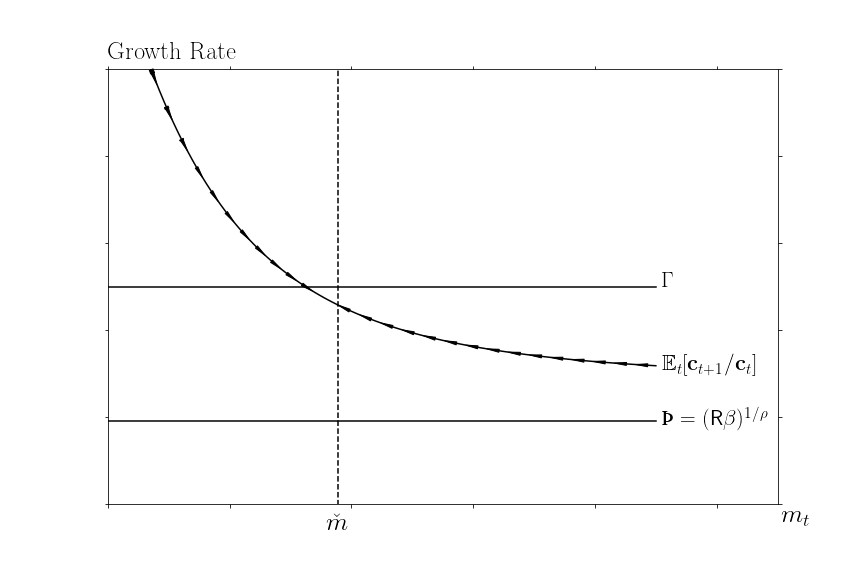
\includegraphics[width=6in]{\FigDir/cGroTargetFig.png}}
\caption{Target $\mRat$, Expected Consumption Growth, and Permanent Income Growth}
\label{fig:cGroTargetFig}
\end{figure}
}{
\begin{figure}[tbp]
\centerline{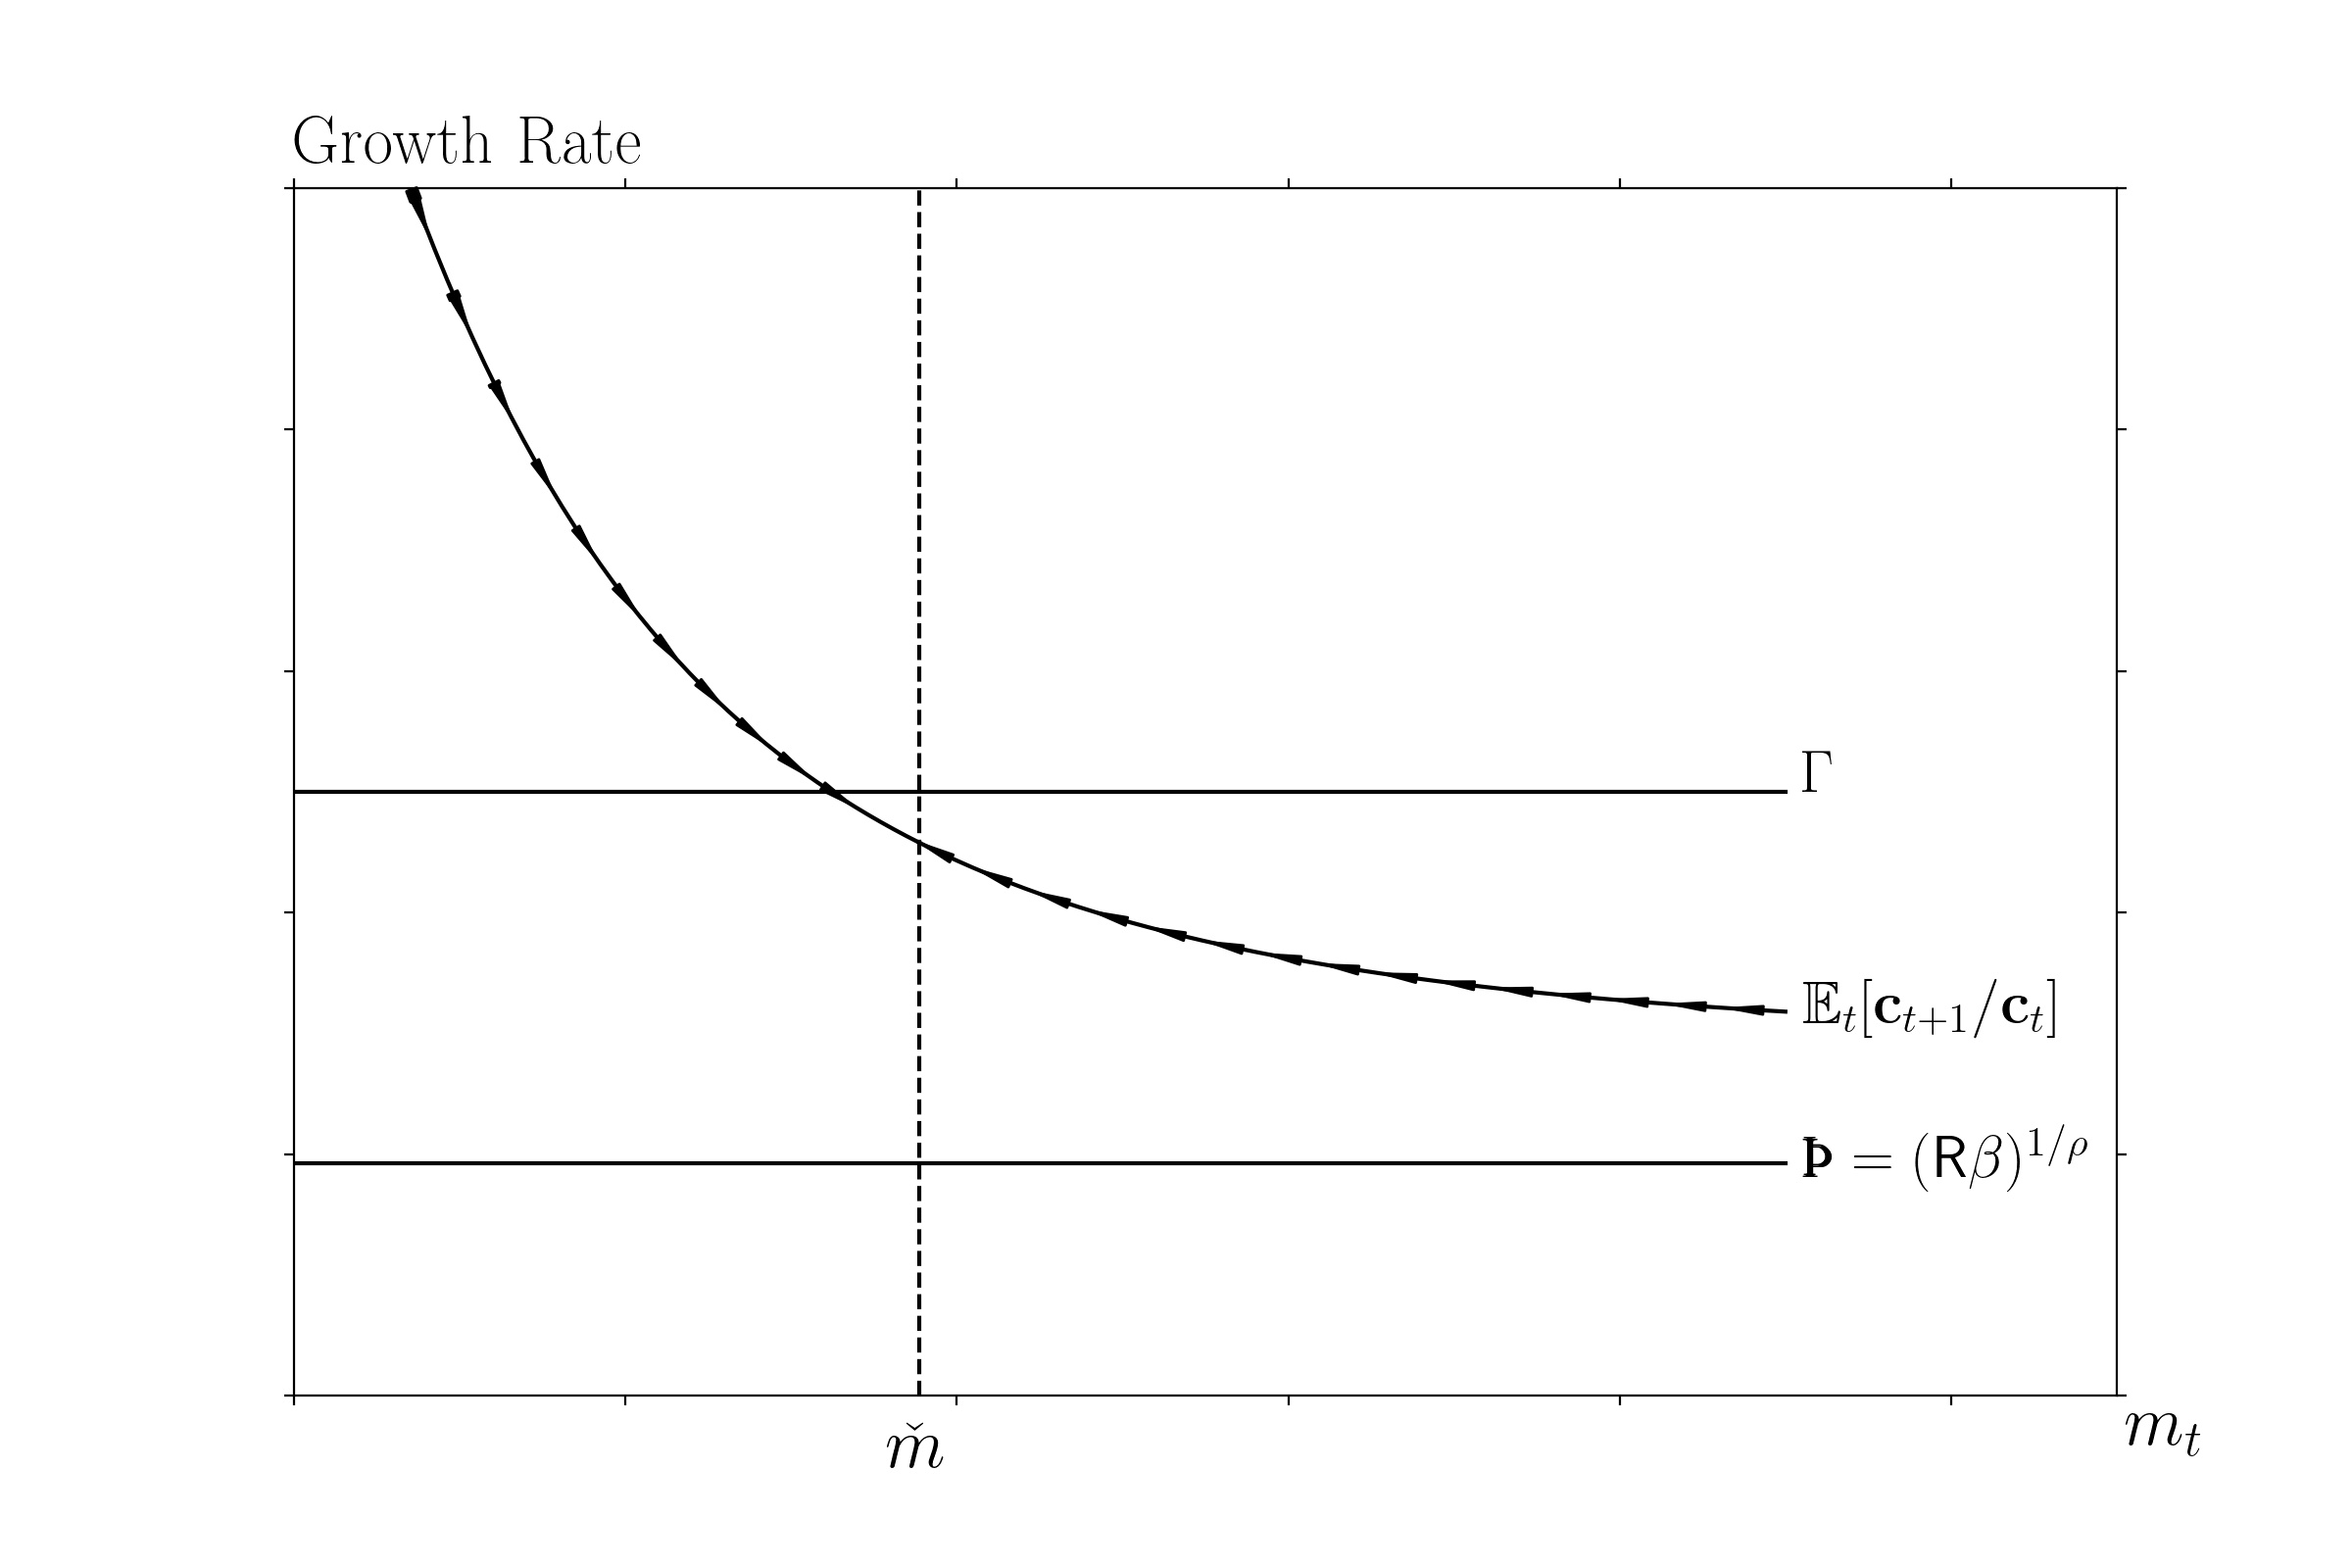
\includegraphics[width=6in]{\FigDir/cGroTargetFig}}
\caption{Target $\mRat$, Expected Consumption Growth, and Permanent Income Growth}
\label{fig:cGroTargetFig}
\end{figure}
}


\hypertarget{LimitsAsmtToInfty}{}
\subsection{Limits as $\mRat_t \uparrow \infty$}

\label{subsec:LimitsAsmtToInfty}

Define
\begin{align}
  \ushort{\cFunc}(\mRat)  & = \MinMPC \mRat \nonumber
\end{align}
which is the solution to an infinite-horizon problem with no noncapital
income
($\tShkAll_{t+n} = 0~\forall~n\geq1$); 
clearly $\ushort{\cFunc}(\mRat)
< \cFunc(\mRat)$, since allowing the possibility of future noncapital
income cannot reduce current consumption.\footnote{We will assume the
  \RIC~holds here and subsequently so that $\MinMPC > 0$; the situation
  is a bit more complex when the \RIC~does not hold.   In that case the bound on consumption is given by the spending
  that would be undertaken by a consumer who faced binding liquidity
  constraints.  Detailed analysis of this special case is not
  sufficiently interesting to warrant inclusion in the paper.}

Assuming the \FHWC~holds, the infinite horizon perfect
foresight solution \eqref{eq:cFuncPFUnc} constitutes an upper
bound on consumption in the presence of uncertainty, since Carroll and
Kimball~\citeyearpar{ckConcavity} show that the introduction of
uncertainty strictly decreases the level of consumption at any $\mRat$.

Thus, we can write
\begin{align}  
  \ushort{\cFunc}(\mRat) < & \cFunc(\mRat)  < \bar{\cFunc}(\mRat) \label{eq:lowerltupper} \\
  1 < & \cFunc(\mRat)/\ushort{\cFunc}(\mRat)  < \bar{\cFunc}(\mRat)/\ushort{\cFunc}(\mRat). \nonumber
\end{align}
But
\begin{align}  \label{eq:limitlowerupper}
  \lim_{m \uparrow \infty} \bar{\cFunc}(\mRat)/\ushort{\cFunc}(\mRat) 
  & = \lim_{m \uparrow \infty} (\mRat -1+ \hRat)/\mRat \nonumber \\
  & = 1, \nonumber
\end{align}
so as $\mRat \uparrow \infty, \cFunc(\mRat)/\ushort{\cFunc}(\mRat)
\rightarrow 1$, and the continuous differentiability and strict
concavity of $\cFunc(\mRat)$ therefore implies
\begin{equation}  \label{eq:limxtoinftycp}
  \lim_{m \uparrow \infty} \cFunc^{\prime}(\mRat) =
  \ushort{\cFunc}^{\prime}(\mRat) = \bar{\cFunc}^{\prime}(\mRat) = \MinMPC \notag
\end{equation}
because any other fixed limit would eventually lead to a level of
consumption either exceeding $\bar{\cFunc}(\mRat)$ or lower than
$\ushort{\cFunc}(\mRat)$.

Figure~\ref{fig:mpclimits} confirms these limits visually.  The top
plot shows the converged consumption function along with its upper and lower bounds,
while the lower plot shows the marginal propensity to consume.
\renewcommand{\figFile}{mpclimits}
\hypertarget{\figFile}{}
\hypertarget{MPCLimits}{}
\begin{figure}
\centerline{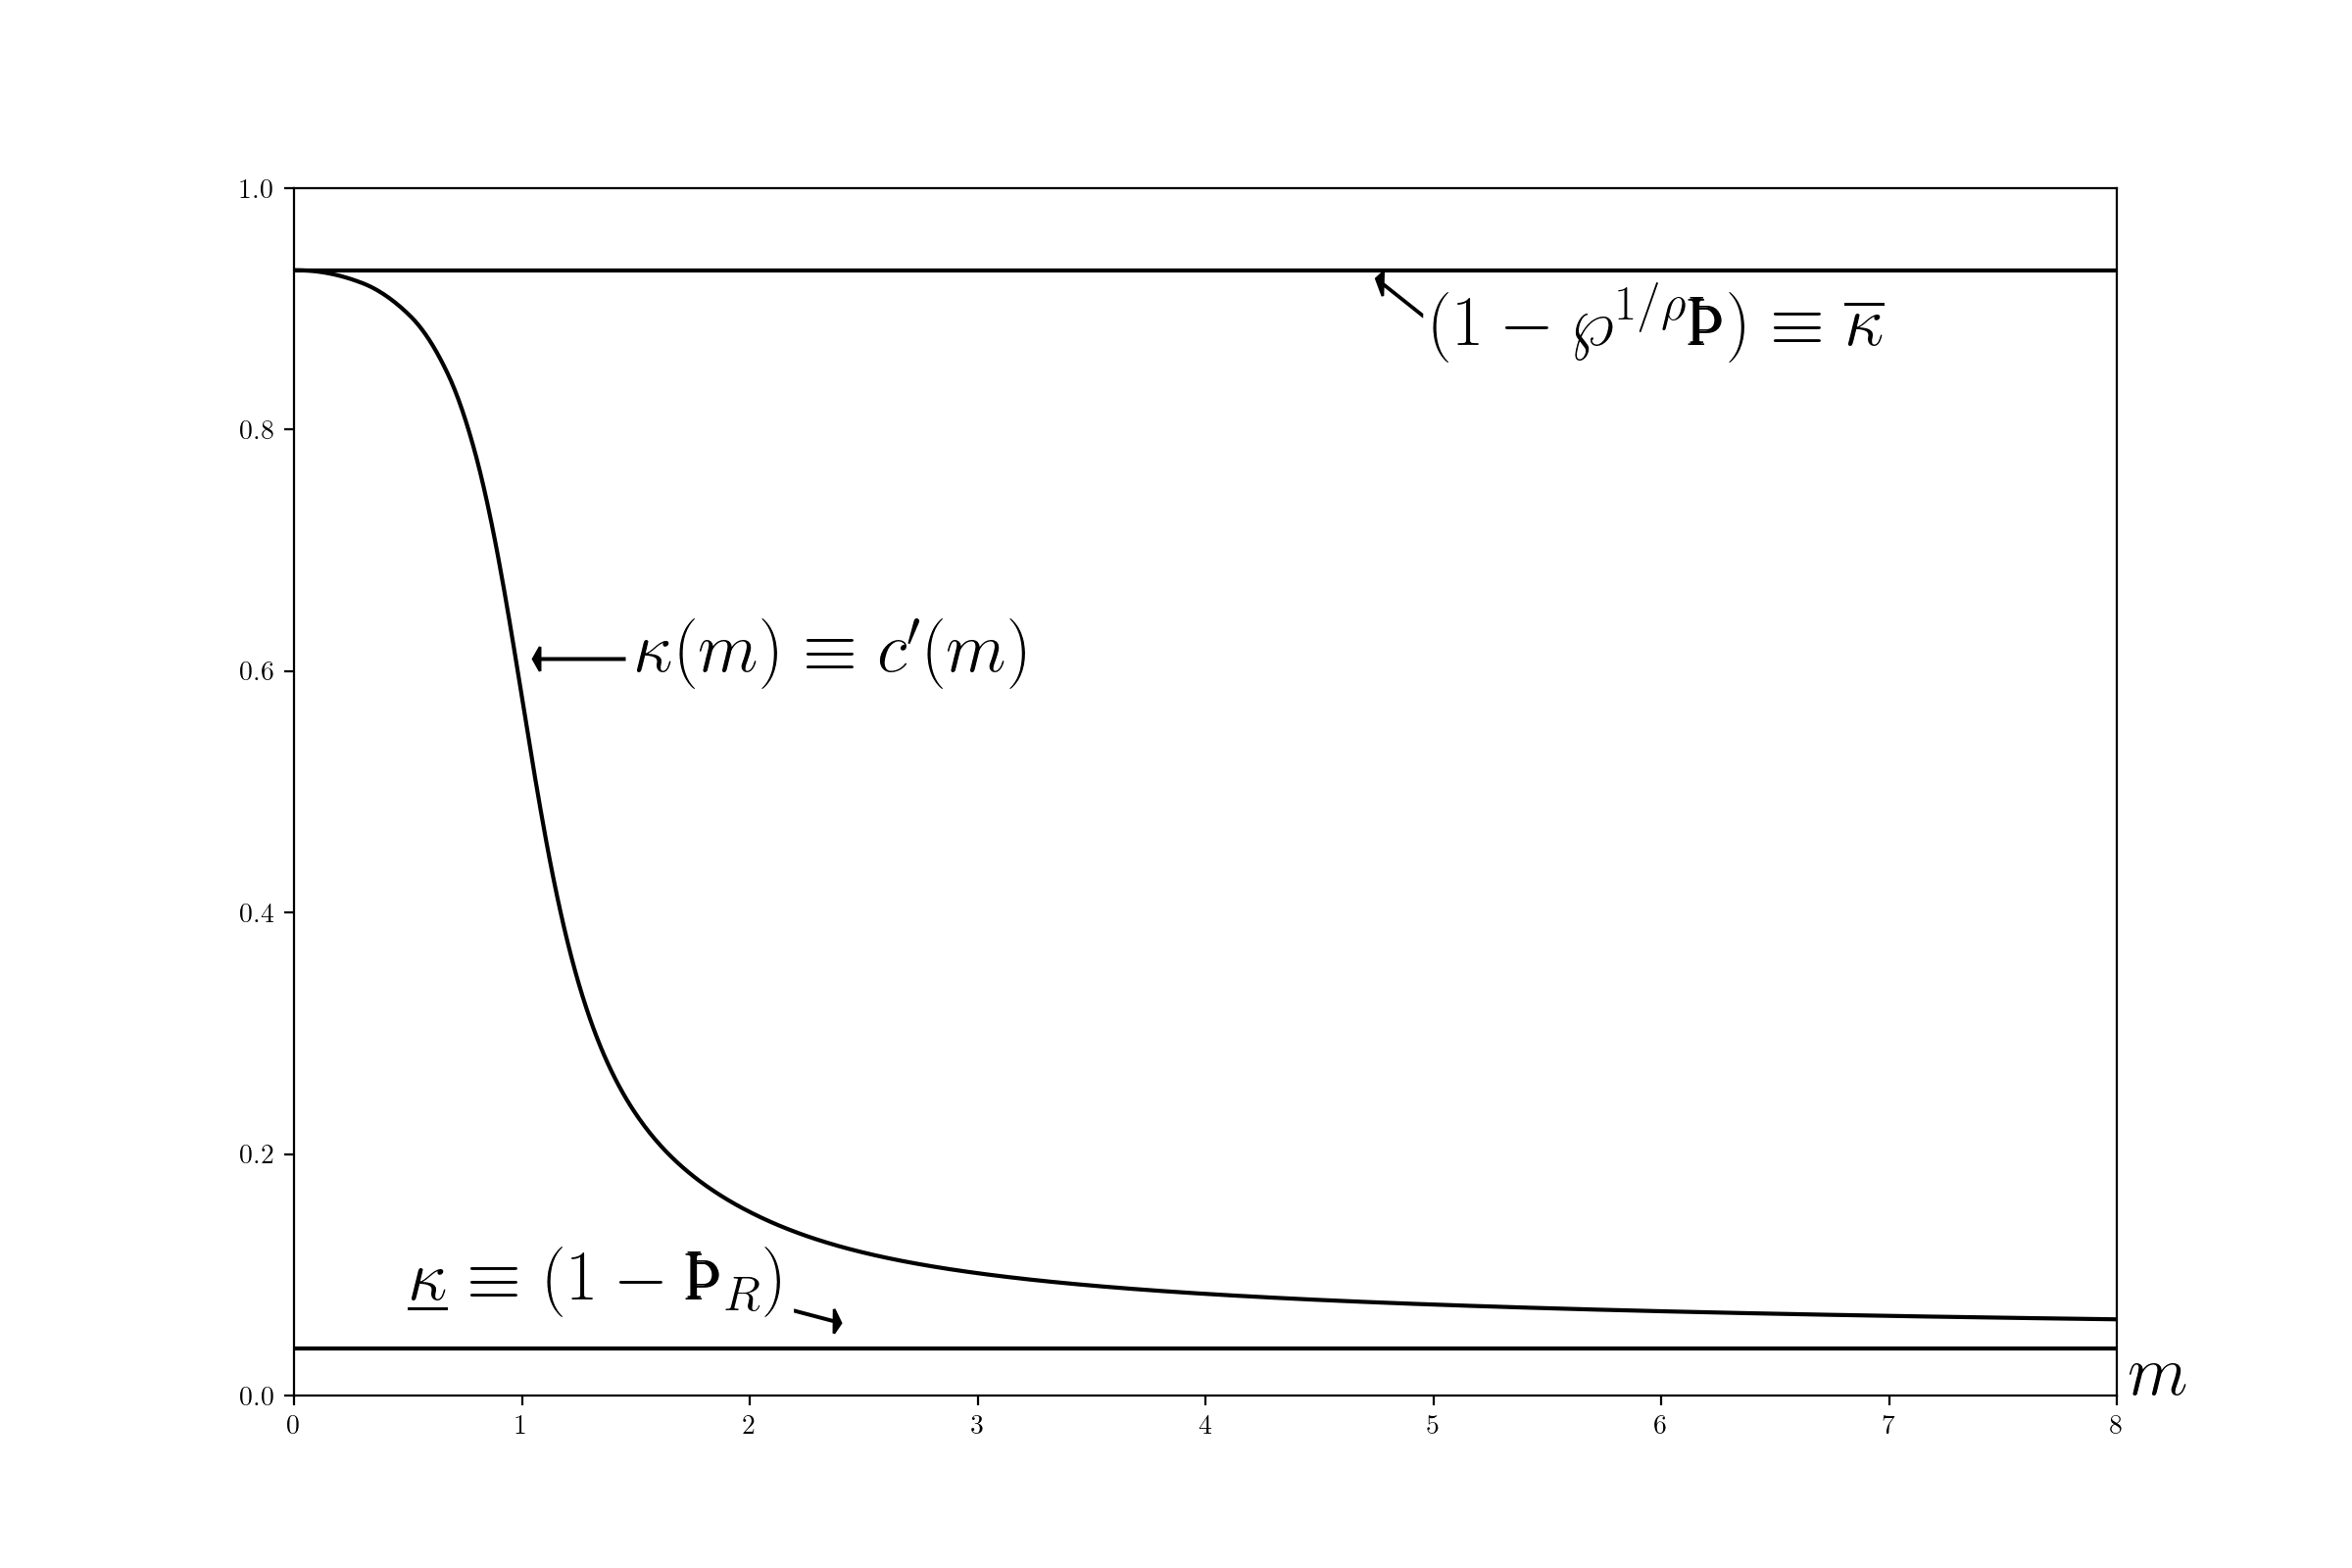
\includegraphics[width=6in]{\FigDir/MPCLimits}}
\caption{Limiting MPC's}
\label{fig:mpclimits}
\end{figure}


\renewcommand{\figFile}{cFuncBounds}
\hypertarget{\figFile}{}
\hypertarget{cFuncBounds}{}
\begin{figure}
\centering
\subfigure[\large Bounds]{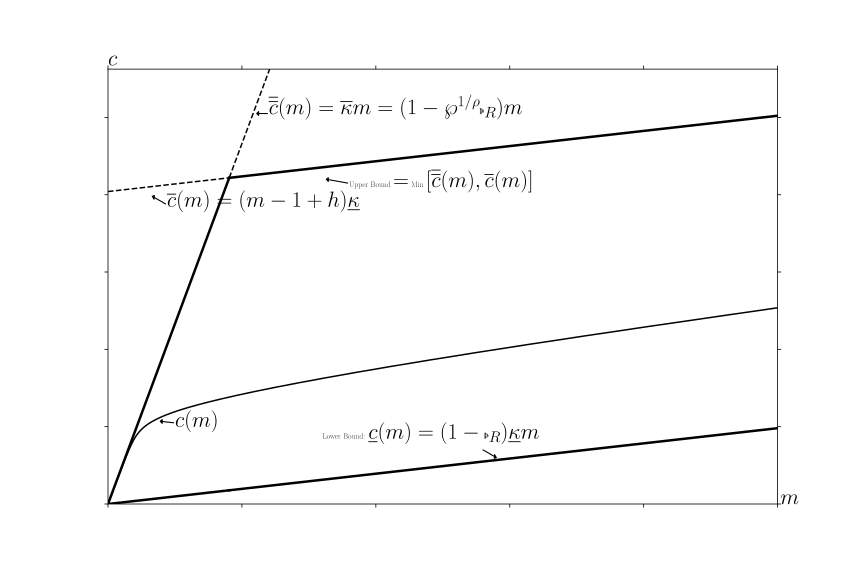
\includegraphics[width=6in]{\FigDir/cFuncBounds}}
\subfigure[\large Target $\mRat$]{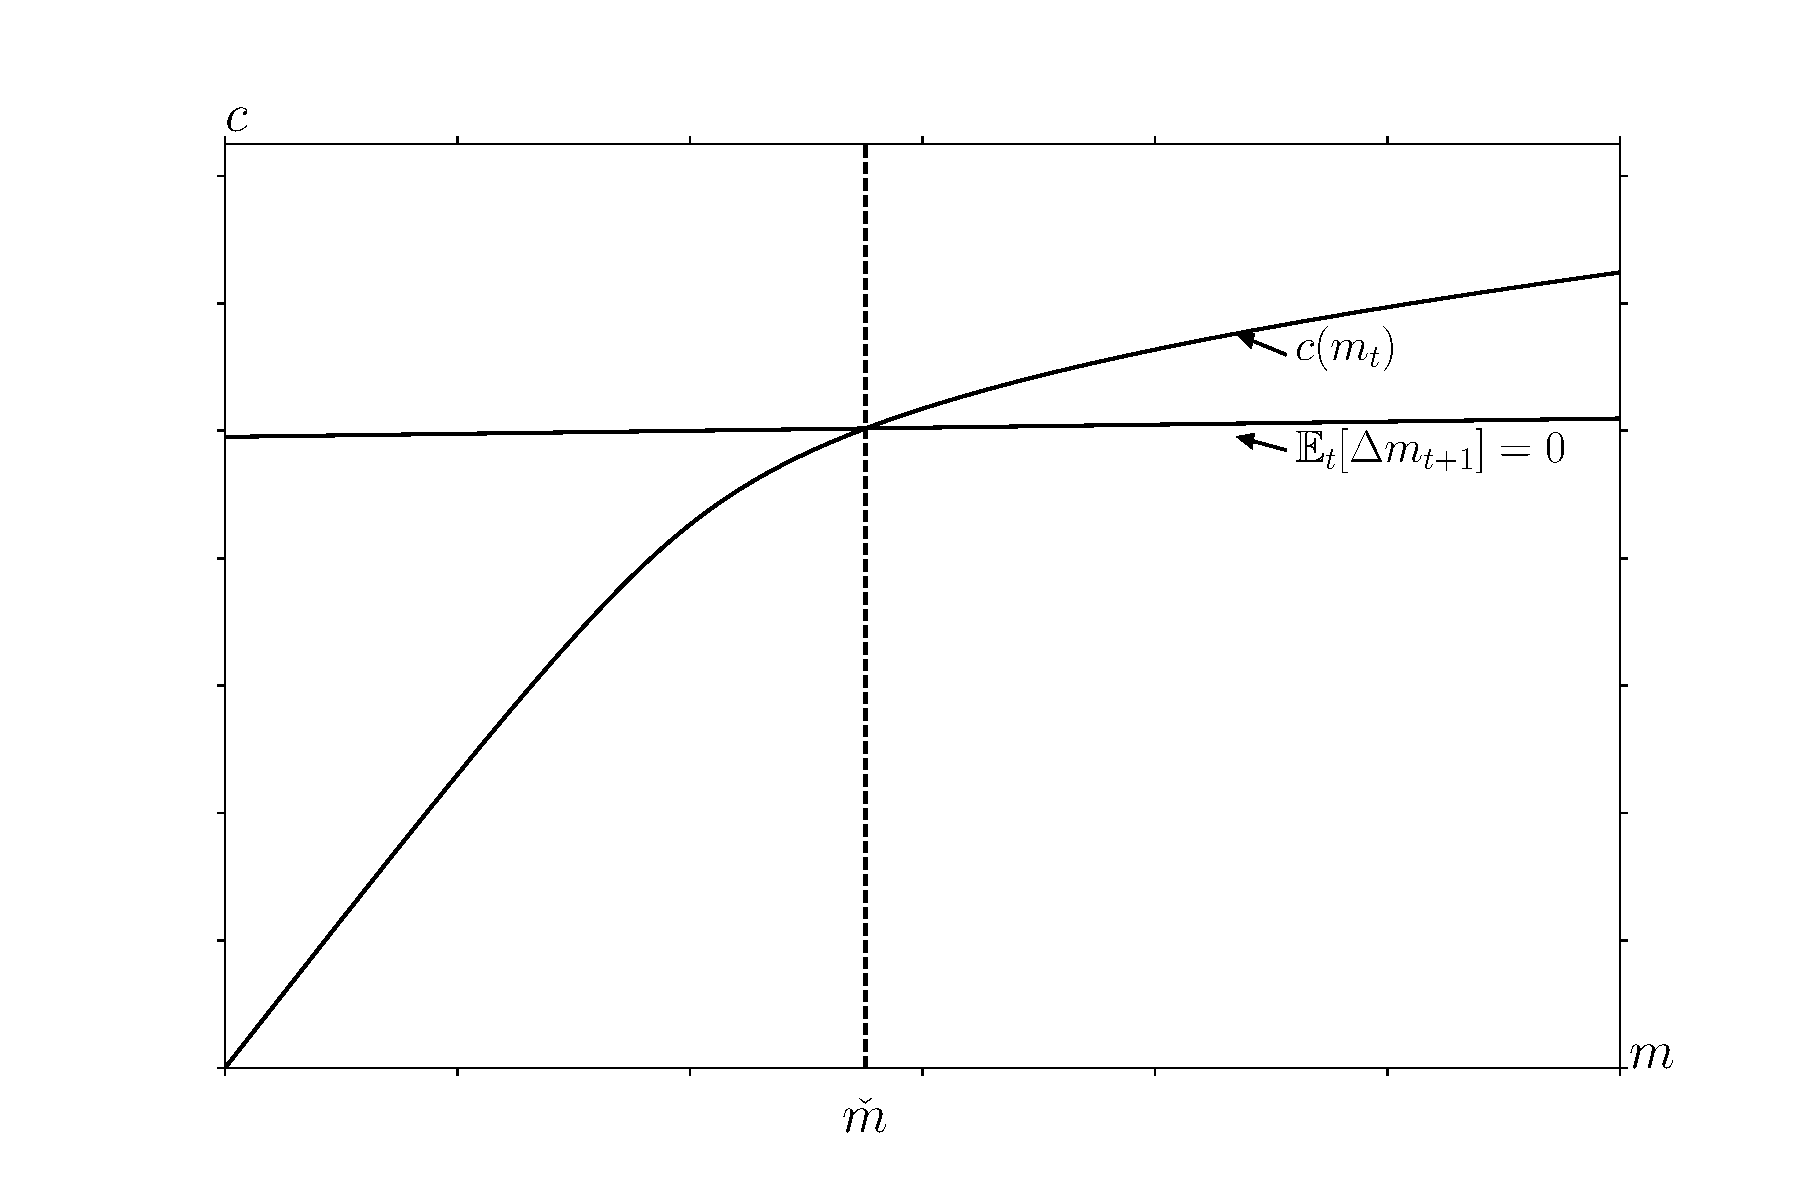
\includegraphics[width=6in]{\FigDir/cRatTargetFig}}
\caption{The Consumption Function}
\label{fig:cFuncBounds}
\end{figure}


Next we establish the limit of the expected consumption growth factor
as $\mRat_{t} \uparrow \infty$:
\begin{align}
  \lim_{\mRat_{t} \uparrow \infty} \Ex_{t}[
  \cLevBF_{t+1}/\cLevBF_{t}]  & = \lim_{\mRat_{t} \uparrow \infty} \Ex_{t}[
                                {\PGro}_{t+1} {\cRat}_{t+1}/c_{t}]. \notag
\end{align}

But
\begin{align*}
  \Ex_{t}[{\PGro}_{t+1} {\ushort{\cRat}}_{t+1}/\bar{\cRat_{t}}] \leq \Ex_{t}[{\PGro}_{t+1} {\cRat}_{t+1}/\cRat_{t}] \leq \Ex_{t}[{\PGro}_{t+1} {\bar{\cRat}}_{t+1}/\ushort{\cRat}_{t}]
\end{align*}
and
\begin{equation}  \label{eq:xttoinfty}
  \lim_{\mRat_t \uparrow \infty} \PGro_{t+1}\ushort{\cFunc}(\mRat_{t+1})/\bar{\cFunc}(\mRat_t) =
  \lim_{\mRat_{t} \uparrow \infty} \PGro_{t+1}\bar{\cFunc}(\mRat_{t+1})/\ushort{\cFunc}(\mRat_t) =
  \lim_{\mRat_{t} \uparrow \infty}\PGro_{t+1} \mRat_{t+1}/\mRat_t,  \notag
\end{equation}
while \hypertarget{xtp1toinfty}{}
\begin{align}  \label{eq:xtp1toinfty}
  \lim_{m_{t} \uparrow \infty} \PGro_{t+1} \mRat_{t+1}/\mRat_t  & = \lim_{m_{t} \uparrow \infty}
                                                                  \left(\frac{\Rfree \aFunc(\mRat_t)+{\PGro}_{t+1}\tShkAll_{t+1}}{\mRat_t}\right)
  \\  & = (\Rfree \DiscFac)^{1/\CRRA} = \Pat
\end{align}
because $\lim_{\mRat_{t}\uparrow \infty} \aFunc^{\prime}(\mRat)=\PatR$\footnote{This is because $\lim_{\mRat_{t}\uparrow \infty} \aFunc(\mRat_{t})/\mRat_{t}=1-\lim_{\mRat_{t}\uparrow \infty} \cFunc(\mRat_{t})/\mRat_{t}=1-\lim_{\mRat_{t}\uparrow \infty}\cFunc^{\prime}(\mRat_{t})=\PatR$.} and
$\PGro_{t+1}\tShkAll_{t+1}/\mRat_{t} \leq (\PGro \bar{\pShk} \bar{\tShkEmp}/\pNotZero )/\mRat_{t}$ which
goes to zero as $\mRat_{t}$ goes to infinity.

Hence we have
\begin{equation}
  {\Pat}  \leq \lim_{\mRat_{t} \uparrow \infty} \Ex_{t}[\cLevBF_{t+1}/\cLevBF_{t}] \leq {\Pat} \nonumber
\end{equation}
so as cash goes to infinity, consumption growth approaches its
value $\Pat$ in the perfect foresight model.

This argument applies equally well to the problem of the restrained
consumer, because as $\mRat$ approaches infinity the constraint becomes
irrelevant (assuming the \FHWC~holds).

\begin{comment}
  Of course, the constraint never becomes irrelevant if human wealth is
  infinite.  We ruled out infinite human wealth at the beginning of this
  section by assuming $\Rfree> \PGro$.  If this finite human wealth
  condition does not hold, it is possible to show that for any finite
  horizon consumer the marginal propensity to consume approaches the
  finite-horizon perfect foresight MPC as wealth approaches infinity.
  However, as the horizon gets longer, the perfect foresight MPC
  approaches zero.  It can be shown therefore that the limiting MPC for
  the converged consumption function approaches (but never reaches)
  zero.  (This is why we chose $\MinMinMPC=0$ if the \FHWC~fails
  in the proofs above.)
\end{comment}

\hypertarget{LimitsAsmtToZero}{}
\subsection{Limits as $\mRat_t \downarrow 0$}

\label{subsec:LimitsAsmtToZero} Now consider the limits of behavior as $\mRat_{t}$ gets
arbitrarily small.

Equation \eqref{eq:MaxMPCInv} shows that the limiting value of
$\MaxMPC$ is
\begin{align}
  \MaxMPC  & = 1-{\Rfree}^{-1}(\pZero  \Rfree\DiscFac)^{1/\CRRA}. \nonumber
\end{align}

Defining $\eFunc(\mRat)=\cFunc(\mRat)/\mRat$ as before we have
\begin{align}
  \lim_{m \downarrow 0} \eFunc(\mRat)  & = (1-\pZero^{1/\CRRA}\PatR) = \MaxMPC \nonumber.
\end{align}

Now using the continuous differentiability of the consumption function
along with L'H\^opital's rule, we have
\begin{comment}
  \begin{align*}
    \eFunc^{\prime}(\mRat)  & = \mRat^{-1} \cFunc^{\prime}(\mRat) - \mRat^{-2} \cFunc(\mRat)
    \\ \mRat \eFunc^{\prime}(\mRat)  & = \cFunc^{\prime}(\mRat) - \cFunc(\mRat)/\mRat
    \\ \cFunc^{\prime}(\mRat)  & = \eFunc(\mRat)+ \mRat \eFunc^{\prime}(\mRat)
  \end{align*}
  and since $0<\eFunc(\mRat)<1$ we have
\end{comment}
\begin{align}
  \lim_{m \downarrow 0} \cFunc^{\prime}(\mRat)  & = \lim_{m \downarrow 0}
                                                  \eFunc(\mRat) = \MaxMPC. \nonumber
\end{align}

Figure~\ref{fig:mpclimits} confirms that the numerical solution method
obtains this limit for the MPC as $\mRat$ approaches zero.

For consumption growth, as $\mRat \downarrow 0$ we have
\begin{align*}
  \lim_{\mRat_{t} \downarrow 0} \Ex_{t}\left[\left(\frac{\cFunc({\mRat}_{t+1})}{\cFunc(\mRat_t)}\right){\PGro}_{t+1}\right]
  & > \lim_{\mRat_{t} \downarrow 0} \Ex_{t}\left[\left(\frac{\ushort{\cFunc}({\mathcal{\mathcal{R}}}_{t+1}\aFunc(\mRat_{t})+{%
    \tShkAll}_{t+1})}{\MaxMPC \mRat_{t}}\right){\PGro}_{t+1}\right]  \notag \\
  & = \pZero \lim_{\mRat_{t} \downarrow 0} \Ex_{t}\left[\left(\frac{\ushort{\cFunc}({\mathcal{\mathcal{R}}}_{t+1}\aFunc(\mRat_{t}))}{\MaxMPC \mRat_{t}}\right){\PGro}_{t+1}\right] \\
  & ~~~~~~ + \pNotZero \lim_{\mRat_{t} \downarrow 0}  \Ex_{t}\left[\left(\frac{\ushort{\cFunc}({\mathcal{\mathcal{R}}}_{t+1}\aFunc(\mRat_{t})+
    \tShkEmp_{t+1}/\pNotZero)}{\MaxMPC \mRat_{t}}\right){\PGro}_{t+1}\right]  \\\notag
  & > \pNotZero \lim_{\mRat_{t} \downarrow 0} \Ex_{t}\left[\left(\frac{\ushort{\cFunc}(
    \tShkEmp_{t+1}/\pNotZero)}{\MaxMPC \mRat_{t}}\right){\PGro}_{t+1}\right] \\
  & = \infty \nonumber
\end{align*}
where the second-to-last line follows because  $\lim_{\mRat_{t} \downarrow 0} \Ex_{t}\left[\left(\frac{\ushort{\cFunc}({\mathcal{\mathcal{R}}}_{t+1}\aFunc(\mRat_{t}))}{\MaxMPC \mRat_{t}}\right){\PGro}_{t+1}\right]$ is positive, and the last line follows because the minimum possible realization of $\tShkEmp_{t+1}$ is $\ushort{\tShkEmp}>0$ so the minimum possible value of expected next-period consumption is positive.\footnote{
  The same arguments establish $\lim_{m \downarrow 0} \Ex_{t}[\cLevBF_{t+1}/\cLevBF_{t}] = \infty$
  for the problem of the restrained consumer.%
}

\hypertarget{onetarget}{}

\subsection{There Exists Exactly One Target Cash-on-Hand Ratio,
  which is Stable}

\label{subsec:onetarget}
\hypertarget{TheoremTarget}{}

We now prove the existence of a target cash-on-hand-to-income ratio $\mTarg$ towards which an agent's $\mRat$ expects to move. (The $\vee$ accent is meant to invoke the fact that this is the value that other $\mRat$'s `point to.') We state the necessary conditions for the existence of $\mTarg$ and its properties in the following theorem.

\begin{theorem}
  \label{thm:target} For the problem defined in section~\ref{subsec:Setup}, 
  if the $\GIC$ \eqref{eq:GIC}, and $\WRIC$ \eqref{eq:WRIC} hold, 
  % \textcolor{red}{$\FHWC$ \eqref{eq:FHWC}},  MVG: Not needed; precautionary motive takes care of it  and $\FVAC$   \eqref{eq:FVAC} hold
  then there exists a unique cash-on-hand-to-income ratio $\mTarg>0$ such that
  \begin{equation}  
    \Ex_t [{\mRat}_{t+1}/\mRat_t] = 1 \mbox{~if~} \mRat_t = \mTarg. 
    \label{eq:mTarget}
  \end{equation}
  Moreover, $\mTarg$ is stable in the sense that
  \begin{align}\label{eq:stability}
    \forall {\mRat}_t\in(0,\mTarg),      \,\,& \Ex_t [{\mRat}_{t+1}] > {\mRat}_t  \\
    \forall {\mRat}_t\in(\mTarg,\infty), \,\,& \Ex_t [{\mRat}_{t+1}] < {\mRat}_t. \notag
  \end{align}

\end{theorem}

The elements of the proof are:
\begin{itemize}
\item Existence and continuity of $\Ex_t [{\mRat}_{t+1}/\mRat_t]$
\item Existence of a point where $\Ex_t [{\mRat}_{t+1}/\mRat_t] = 1$
\item $\Ex_t [{\mRat}_{t+1}]-\mRat_{t}$ is monotonically decreasing
\end{itemize}

\subsubsection{Existence and Continuity of $\Ex_t [{\mRat}_{t+1}/\mRat_t]$.}
The consumption function exists because we have imposed the conditions (the $\WRIC$ and $\FVAC$) that theorem~\ref{thm:contmap} establishes are sufficient for its existence.  (Indeed, Appendix~\ref{sec:CIsTwiceDifferentiable} shows that $\cFunc(\mRat)$ is not just continuous, but twice continuously differentiable.)

Section~\ref{sec:cExists} shows that for all $t$, $\aRat_{t-1} = {\mRat}_{t-1} -  \cRat_{t-1} > 0$.  Since ${\mRat}_{t}= {\aRat}_{t-1} \Rnorm_{t} + \yRat_{t}$, even if $\yRat_{t}$ takes on its minimum value of 0, $\aRat_{t-1} \Rnorm_{t} > 0$, since both $\aRat_{t-1}$ and $\Rnorm_{t}$ are strictly positive under our foregoing assumptions.  With $\mRat_{t} > 0$, the ratio $\Ex_t [{\mRat}_{t+1}/\mRat_t]$ inherits continuity (and, for that matter, continuous differentiability) from the consumption function.

\subsubsection{Existence of a point where $\Ex_t [{\mRat}_{t+1}/\mRat_t]=1$.}
The logic in section~\ref{subsec:LimitsAsmtToZero} showing that $\lim_{\mRat_t \downarrow 0} 
\Ex_t [{\cRat}_{t+1}/\cRat_t] = \infty$ transparently implies the same proposition for $\mRat_{t}$: $\lim_{\mRat_{t}\downarrow 0} \Ex_{t}[\mRat_{t+1}] > 0$ so the ratio is unbounded. 

The limit as $\mRat_{t}$ goes to infinity is
\begin{align}
  \lim_{\mRat_{t} \uparrow \infty} \Ex_{t}[{\mRat}_{t+1}/\mRat_{t}]  & =   
                                                                       \lim_{\mRat_{t} \uparrow \infty} 
                                                                       \Ex_{t}\left[\frac{{\mathcal{\mathcal{R}}}_{t+1}\aFunc(\mRat_{t})+{\tShkAll}_{t+1}}{\mRat_{t}}\right] \notag 
  \\  & = \Ex_{t}[(\Rfree/{\PGro}_{t+1})\PatR]
  \\  & = \Ex_{t}[{\Pat}/{\PGro}_{t+1}] \notag
  \\  & < 1 \notag
\end{align}
where the last two lines are merely a restatement of the \GIC~\eqref{eq:GIC}.

The Intermediate Value Theorem tells us that if $\Ex_t [{\mRat}_{t+1}/\mRat_t]$ is continuous, and takes on values above and below 1, there must be at least one point at which it is equal to one.

\subsubsection{$\Ex_t [{\mRat}_{t+1}] -\mRat_t$ is monotonically decreasing.}

Now define \providecommand{\difFunc}{\pmb{\zeta}} $\difFunc(\mRat_t) \equiv 
\Ex_t[\mRat_{t+1}] - \mRat_t$ and note that
\begin{align}\label{eq:difRatioEquiv}
  \difFunc(\mRat_t) < 0 &\leftrightarrow \Ex_t[{\mRat}_{t+1}/\mRat_t] < 1 
                          \nonumber\\
  \difFunc(\mRat_t) = 0 &\leftrightarrow \Ex_t[{\mRat}_{t+1}/\mRat_t] = 1\\
  \difFunc(\mRat_t) > 0 &\leftrightarrow \Ex_t[{\mRat}_{t+1}/\mRat_t] > 
                          1,\nonumber
\end{align}
so that $\difFunc(\mTarg)=0$. Our goal is to prove that $\difFunc(\bullet)$ is strictly 
decreasing on $(0,\infty)$ using the fact that
\begin{align}
  \difFunc^{\prime}(\mRat_{t}) \equiv  \left( \frac{d}{d\mRat_{t}}\right) \difFunc(\mRat_t)  & = \Ex_{t}\left[
                                                                                               \left( \frac{d}{d\mRat_{t}}\right) \left( 
                                                                                               {\Rnorm}_{t+1}(\mRat_{t}-\cFunc(\mRat_{t}))+%
                                                                                               {\tShkAll}_{t+1} - {\mRat}_t\right) \right] \label{eq:difFuncDecreases} \\
                                                                                             & = \bar{\Rnorm}\left(1-\cFunc^{\prime}({\mRat}_t)\right) - 1.  \notag
\end{align}

Note that the statement of theorem~\ref{thm:target} did not require the {\RIC} to hold.  Now, we show that (given our other assumptions) $\difFunc^{\prime}(\mRat)$ is decreasing (but for different reasons) whether the {\RIC} holds or fails (\cncl{\RIC}).

\textbf{If {\RIC} holds}. Equation~\ref{eq:MinMPCDef} indicates that if the {\RIC} holds, then $\MinMPC >0$.  We show at the bottom of Section~\ref{sec:WRIC} that if the {\RIC} holds then $0 < \MinMPC < \cFunc^{\prime}(\mRat_{t}) < 1$ so that 
\begin{align*}
  \bar{\Rnorm}\left(1-\cFunc^{\prime}({\mRat}_t)\right) - 1 & <  \bar{\Rnorm}(1-\underbrace{(1-\PatR)}_{\MinMPC}) - 1  \\
                                                            & = \bar{\Rnorm}\PatR - 1 \\
                                                            & = \Ex_{t}\left[\frac{\Rfree}{\PGro \pShk}\frac{\Pat}{\Rfree}\right] - 1 \\
                                                            & = \underbrace{\Ex_{t}\left[\frac{\Pat}{\PGro \pShk}\right]}_{= \PatPGroAdj} - 1 
\end{align*}
which is negative because the {\GIC} says $\PatPGroAdj < 1$.  

\textbf{If {\RIC} fails.}
Under \cncl{\RIC}, recall that $\lim_{\mRat \uparrow \infty} \cFunc^{\prime}(\mRat) = 0$.  Concavity of the consumption function means that $\cFunc^{\prime}$ is a decreasing function, so everywhere 
\begin{align*}
  \bar{\Rnorm}\left(1-\cFunc^{\prime}({\mRat}_t)\right) & < \bar{\Rnorm}
\end{align*}
which means that $\difFunc^{\prime}(\mRat_{t})$ from \eqref{eq:difFuncDecreases} is guaranteed to be negative if
\begin{align}
  \bar{\Rnorm} \equiv \Ex_{t}\left[\frac{\Rfree}{\PGro \pShk}\right] & < 1  \label{eq:RbarBelowOne}
\end{align}
But the combination of the {\GIC} holding and the {\RIC} failing can be written:
\begin{align*}
  \overbrace{\Ex_{t}\left[\frac{\Pat}{\PGro \pShk}\right]}^{\PatPGroAdj} & < 1 < \overbrace{\frac{\Pat}{\Rfree}}^{{\PatR}},
\end{align*}
and multiplying all three elements by $\Rfree/\Pat$ gives 
\begin{align*}
  \Ex_{t}\left[\frac{\Rfree}{\PGro \pShk}\right] & < \Rfree/\Pat < 1
\end{align*}
which satisfies our requirement in \eqref{eq:RbarBelowOne}.\footnote{An interesting sidenote is that \eqref{eq:RbarBelowOne} is a close cousin to the {\FHWC}: instead of $\Rfree/\PGro < 1$ we have $(\Rfree/\PGro)\InvEpShkInv < 1$.}

% where the bound on the marginal propensity to consume in the third line  is guaranteed by the $RIC$ \eqref{eq:RIC} (see section~\ref{subsec:LimitsAsmtToInfty}) \textcolor{red}{Is the FHWC needed?}. Therefore, we can be sure that $\difFunc(\bullet)$ crosses 0 exactlyonce at $\mTarg$, and through \eqref{eq:difRatioEquiv} this implies that the target is unique. Additionally, we can conclude that$\difFunc({\mRat}_t)>0$ for ${\mRat}_t<\mTarg$ and $\difFunc({\mRat}_t)>0$ for ${\mRat}_t > \mTarg$, which coupled with \eqref{eq:difRatioEquiv} yields our desired stability result \eqref{eq:stability}.

The foregoing arguments rely on the continuous differentiability of
$\cFunc(\mRat)$, so the arguments do not directly go through for the
restrained consumer's problem in which the existence of liquidity
constraints can lead to discrete changes in the slope
$\cFunc^{\prime}(\mRat)$ at particular values of $\mRat$. But we can
use the fact that the restrained model is the limit of the baseline
model as $\pZero \downarrow 0$ to conclude that there is likely a
unique target cash level even in the restrained model.

If consumers are sufficiently impatient, the limiting target level in the
restrained model will be $\mTarg = \Ex_{t}[{\tShkAll}_{t+1}] = 1$. That
is, if a consumer starting with $\mRat = 1$ will save nothing, ${\aFunc}(1)=0$,
then the target level of $\mRat$ in the restrained model will be 1; if a
consumer with $\mRat=1$ would choose to save something, then the target
level of cash-on-hand will be greater than the expected level of income.

\hypertarget{cGroLTpGro}{}
\subsection{Expected Consumption Growth at Target $\mRat$ Is Less than
  Expected Permanent Income Growth}

\label{subsec:expcgrowth} In Figure~\ref{fig:cGroTargetFig} the intersection of
the target cash-on-hand ratio locus at $\mTarg$ with the expected consumption
growth curve lies below the intersection with the horizontal line
representing the growth rate of expected permanent income. This can be
proven as follows.

Strict concavity of the consumption function implies that if $\Ex_{t}[{\mRat}_{t+1}] = \mTarg = \mRat_{t}$ then
\begin{align}
  \Ex_{t}\left[\frac{{\PGro}_{t+1} \cFunc({\mRat}_{t+1})}{\cFunc(\mRat_{t})}
  \right]  & < \Ex_{t}\left[\left(\frac{{\PGro}_{t+1}
             (\cFunc(\mTarg)+\cFunc^{\prime}(\mTarg)({\mRat}_{t+1}-\mTarg))}{\cFunc(\mTarg)}\right)\right]  \nonumber \\
           & = \Ex_{t}\left[{\PGro}_{t+1} \left(1+\left(\frac{\cFunc^{\prime}(\mTarg)}{%
             \cFunc(\mTarg)}\right)({\mRat}_{t+1}-\mTarg)\right)\right]  \nonumber  \\
           & = \PGro + \left(\frac{\cFunc^{\prime}(\mTarg)}{\cFunc(\mTarg)}\right)\Ex_{t}\left[ {\PGro}_{t+1}\left({\mRat}_{t+1}-\mTarg\right)\right]  \nonumber \\
           & = \PGro + \left(\frac{\cFunc^{\prime}(\mTarg)}{\cFunc(\mTarg)}\right)\left[
             \Ex_{t}[ \PGro_{t+1}]\underbrace{\Ex_{t}[
             {\mRat}_{t+1}-\mTarg]}_{=0}+\mbox{cov}_{t}( {\PGro}_{t+1},{\mRat}_{t+1})\right]
             \label{eq:covcgrow}
\end{align}
and since $\mRat_{t+1} = (\Rfree/\PGro_{t+1}) \aFunc(\mTarg)+\tShkAll_{t+1}$ and
$\aFunc(\mTarg)>0$ it is clear that
cov$_{t}({\PGro}_{t+1},{\mRat}_{t+1})<0$ which implies that
the entire term added to $\PGro$ in \eqref{eq:covcgrow} is negative, as
required.

\hypertarget{dcgdxneg}{}
\subsection{Expected Consumption Growth Is a Declining Function of $\mRat_{t}$ (or Is It?)}
\label{subsec:dcgdxneg}

Figure~\ref{fig:cGroTargetFig} depicts the expected consumption growth factor as a strictly
declining function of the cash-on-hand ratio. To investigate this,
define
\begin{align*}
  \pmb{\Upsilon}(\mRat_{t})  & \equiv  \PGro_{t+1} \cFunc(\Rnorm_{t+1}\aFunc(\mRat_{t})+\tShkAll_{t+1})/\cFunc(\mRat_{t})  = \cLevBF_{t+1}/\cLevBF_{t}
\end{align*}
and the proposition in which we are interested is

\begin{align}
  (d/d\mRat_{t})\Ex_{t}[\underbrace{\pmb{\Upsilon}(\mRat_{t})}_{\equiv \pmb{\Upsilon}_{t+1}}]  & < 0  \nonumber
\end{align}
or differentiating through the expectations operator, what we want is
\begin{align}
  \Ex_{t}\left[\PGro_{t+1} \left(\frac{\cFunc^{\prime}(\mRat_{t+1})\Rnorm_{t+1}\aFunc^{\prime}(\mRat_{t})\cFunc(\mRat_{t})-\cFunc(\mRat_{t+1})\cFunc^{\prime}(\mRat_{t})}{\cFunc(\mRat_{t})^{2}}\right)\right]  & < 0 \label{eq:kappaPrimeLT0}.
\end{align}

Henceforth indicating appropriate arguments by the corresponding
subscript (e.g.\ $\cFunc_{t+1}^{\prime} \equiv \cFunc^{\prime}(\mRat_{t+1})$), since
$\PGro_{t+1}\Rnorm_{t+1}=\Rfree$, the portion of the LHS of equation \eqref{eq:kappaPrimeLT0} in brackets can be manipulated to yield
\begin{align}
  \cFunc_{t} \pmb{\Upsilon}^{\prime}_{t+1}  & = \cFunc^{\prime}_{t+1}\aFunc^{\prime}_{t}\Rfree-\cFunc^{\prime}_{t} \PGro_{t+1} \cFunc_{t+1}/\cFunc_{t} \nonumber
  \\  & = \cFunc^{\prime}_{t+1}\aFunc^{\prime}_{t}\Rfree-\cFunc^{\prime}_{t} \pmb{\Upsilon}_{t+1} \label{eq:cPrimek}
        .
\end{align}

Now differentiate the Euler equation with respect to $\mRat_{t}$:
\begin{align}
  1  & = \Rfree \DiscFac \Ex_{t}[ \pmb{\Upsilon}_{t+1}^{-\CRRA}] \notag
  \\ 0  & = \Ex_{t}[\pmb{\Upsilon}_{t+1}^{-\CRRA-1} \pmb{\Upsilon}_{t+1}^{\prime}] \notag
  \\  & = \Ex_{t}[\pmb{\Upsilon}_{t+1}^{-\CRRA-1}]\Ex_{t}[\pmb{\Upsilon}_{t+1}^{\prime}]+\mbox{cov}_{t}(\pmb{\Upsilon}_{t+1}^{-\CRRA-1},\pmb{\Upsilon}_{t+1}^{\prime}) \notag
  \\ \Ex_{t}[\pmb{\Upsilon}_{t+1}^{\prime}]  & = -\mbox{cov}_{t}(\pmb{\Upsilon}_{t+1}^{-\CRRA-1},\pmb{\Upsilon}_{t+1}^{\prime})/\Ex_{t}[\pmb{\Upsilon}_{t+1}^{-\CRRA-1}] \label{eq:covgen}
\end{align}
but since $\pmb{\Upsilon}_{t+1} > 0$ we can see from \eqref{eq:covgen} that \eqref{eq:kappaPrimeLT0} is equivalent to
\begin{align}
  \mbox{cov}_{t}(\pmb{\Upsilon}_{t+1}^{-\CRRA-1},\pmb{\Upsilon}_{t+1}^{\prime})  & > 0 \nonumber
\end{align}
which, using \eqref{eq:cPrimek}, will be true if
\begin{align}
  \mbox{cov}_{t}(\pmb{\Upsilon}_{t+1}^{-\CRRA-1},\cFunc^{\prime}_{t+1}\aFunc^{\prime}_{t}\Rfree - \cFunc^{\prime}_{t}\pmb{\Upsilon}_{t+1})  & > 0 \notag
\end{align}
which in turn will be true if both
\begin{align}
  \mbox{cov}_{t}(\pmb{\Upsilon}_{t+1}^{-\CRRA-1},\cFunc^{\prime}_{t+1} )  & > 0 \notag
\end{align}
and
\begin{align*}
  \mbox{cov}_{t}(\pmb{\Upsilon}_{t+1}^{-\CRRA-1},\pmb{\Upsilon}_{t+1})  & < 0. \notag
\end{align*}

The latter proposition is obviously true under our assumption $\CRRA > 1$.  The former will be true if
\begin{align*}
  \mbox{cov}_{t}\left((\PGro \pShk_{t+1} \cFunc(\mRat_{t+1}))^{-\CRRA-1},\cFunc^{\prime}(\mRat_{t+1}) \right)  & > 0 \nonumber.
\end{align*}

The two shocks cause two kinds of variation in $\mRat_{t+1}$.
Variations due to $\tShkAll_{t+1}$ satisfy the proposition, since a
higher draw of $\tShkAll$ both reduces $c_{t+1}^{-\CRRA-1}$ and
reduces the marginal propensity to consume.  However, permanent shocks
have conflicting effects.  On the one hand, a higher draw of
$\pShk_{t+1}$ will reduce $\mRat_{t+1}$, thus increasing both
$c_{t+1}^{-\CRRA-1}$ and $c_{t+1}^{\prime}$.  On the other hand, the
$c_{t+1}^{-\CRRA-1}$ term is multiplied by $\PGro \pShk_{t+1}$, so the
effect of a higher $\pShk_{t+1}$ could be to decrease the first term
in the covariance, leading to a negative covariance with the second
term.  (Analogously, a lower permanent shock $\pShk_{t+1}$ can also
lead a negative correlation.)

The software archive associated with this paper presents an example in
which this perverse effect dominates.  However, extreme assumptions
were required (in particular, a very small probability of the
zero-income shock) and the region in which
$\pmb{\Upsilon}_{t+1}^{\prime} > 0$ was tiny.  In practice, for
plausible parametric choices,
$\Ex_{t}[\pmb{\Upsilon}_{t+1}^{\prime}]<0$ should generally hold.

% \ifthenelse{\boolean{showBody}}{

\hypertarget{The-Aggregate-and-Idiosyncratic-Relationship-Between-Consumption-Growth-and-Income-Growth}{}
\section{The Aggregate and Idiosyncratic Relationship Between
  Consumption Growth and Income Growth}

This section examines the behavior of large collections of buffer-stock consumers with identical parameter values. Such a collection can be thought of as either a subset of the population within a single country (say, members of a given education or occupation group), or as the whole population in a small open economy.\footnote{We will continue to take the aggregate interest rate as exogenous and constant. It is also possible, and only slightly more difficult, to solve for the steady-state of a closed-economy version of the model where the interest rate is endogenous.}

We have assumed infinite horizons.  In practice, aggregative (macroeconomic) models of this kind usually incorporate mortality in some fashion. We omit mortality here because its incorporation in standard ways does not modify any of the derivations; but mortality can have important quantitative implications, which are discussed briefly in Section~\ref{sec:Mortality-And-Redistribution}

Formally, we assume a continuum of {\it ex ante} identical households
on the unit interval, with constant total mass normalized to one and
indexed by $i \in [0,1]$, all behaving according to the model
specified above.\footnote{One inconvenient aspect of the model as
  specified is that it does not exhibit a stationary distribution of
  idiosyncratic permanent noncapital income; the longer the economy lasts, the wider is the
  distribution.  This problem can be remedied by assuming a constant
  probability of death, and replacing deceased households with
  newborns whose initial idiosyncratic permanent income matches the
  mean idiosyncratic permanent income of the population.  For a fully
  worked-out general equilibrium version of such a model, see \cite{BSinKS}.}

Szeidl~\citeyearpar{szeidlInvariant} proves that such a
population will be characterized by an invariant
distribution of $\mRat$ that induces invariant distributions for $\cRat$ and
$\aRat$; designate these $\mathcal{F}^{\mRat}$, $\mathcal{F}^{\aRat}$, and
$\mathcal{F}^{\cRat}$.\footnote{Szeidl's proof supplants simulation evidence of ergodicity
  that appeared in an earlier version of this paper.}

\hypertarget{Consumption-and-Income-Growth-at-the-Household-Level}{}
\subsection{Consumption and Income Growth at the Household Level}

It is useful to define the operator $\Mean\left[\bullet\right]$ which yields the mean value of its argument in the population, as distinct from the expectations operator $\Ex\left[\bullet\right]$ which represents beliefs about the future.

An economist with a microeconomic dataset could calculate the average
growth rate of idiosyncratic consumption, and would find
\begin{align*}
  \Mean\left[\Delta \log \cLevBF_{t+1}\right]  & = \Mean\left[ \log {\cRat}_{t+1}\pLevBF_{t+1} - \log c_{t}\pLevBF_{t}\right]  \notag \\
                                               & = \Mean\left[ \log \pLevBF_{t+1}- \log \pLevBF_{t} + \log {\cRat}_{t+1} - \log c_{t}\right]  \notag \\
                                               & = \Mean\left[ \log \pLevBF_{t+1}- \log \pLevBF_{t}\right] + \Mean\left[ \log {\cRat}_{t+1} - \log c_{t}\right]  \notag \\
                                               & = (\gamma - \sigma^{2}_{\pshk}/2) + \Mean[\log \cRat_{t+1} - \log \cRat_{t}] \\
                                               & = (\gamma - \sigma^{2}_{\pshk}/2)
\end{align*}
where $\gamma=\log \PGro$ and the last equality follows because the invariance of
$\mathcal{F}^{\cRat}$ (see \cite{szeidlInvariant}) means that $\Mean\left[ \log
  {\cRat}_{t+n}\right] = \Mean\left[ \log
  c_{t}\right]$.\footnote{Papers in the simulation literature have
  observed an approximate equivalence between the average growth rates
  of idiosyncratic consumption and permanent income, but formal proof
  was not possible until Szeidl's proof of ergodicity.}

Thus, in a population that has reached its invariant distribution, the growth
rate of idiosyncratic log consumption matches the growth rate of idiosyncratic log permanent income.

\ShorterYN{}{
  \hypertarget{Growth-Rates-of-Aggregate-Income-and-Consumption}{}
  \subsection{Growth Rates of Aggregate Income and Consumption}
  \label{subsec:cGroEqPGroQ}

  Attanasio and Weber~\citeyearpar{aw95} point out that
  concavity of the consumption function (or other nonlinearities) can
  imply that it is quantitatively important to distinguish between the
  growth rate of average consumption and the average growth rate of
  consumption.\footnote{Since we assume number of the households are
    normalized to 1, aggregate and average variables are identical.}  We
  have just examined the average growth rate; we now examine the growth
  rate of the average.

  Using boldface capital letters for aggregate
  variables, the growth factor for aggregate income is given by:
  \begin{align*}
    \YLevBF_{t+1}/\YLevBF_{t}  & = \Mean\left[\tShkAll_{t+1}\PGro \pShk_{t+1}\pLevBF_{t}\right]/\Mean\left[\pLevBF_{t}\tShkAll_{t}\right]  \\
                               & = \PGro
  \end{align*}
  because of the independence assumptions we have made about $\tShkAll$ and $\pShk$.

  The growth factor for aggregate assets is:
  \begin{align*}
    \left(\frac{\ALevBF_{t+1}}{\ALevBF_{t}}\right)  & = \frac{\Mean[a_{t+1} \pLevBF_{t+1}]}{\Mean[a_{t} \pLevBF_{t}]}   \\ 
                                                    & = \PGro \left[\frac{\Mean[a_{t+1}\pLevBF_{t}\psi_{t+1}]}{\Mean[a_{t}\pLevBF_{t}]}\right] \\
                                                    % & = \PGro \left[\frac{\Mean[(a_{t+1}/a_{t})a_{t}\pLevBF_{t}\psi_{t+1}]}{\Mean[a_{t}\pLevBF_{t}]}\right] \\
                                                    % & = \PGro \left[\frac{\Mean[(\psi_{t+1}a_{t+1}/a_{t})]\Mean[a_{t}\pLevBF_{t}]+\cov(\psi_{t+1}a_{t+1}/a_{t},a_{t}\pLevBF_{t})}{\Mean[a_{t}\pLevBF_{t}]}\right] \\
                                                    & = \PGro \left[\frac{\Mean[(a_{t}+(a_{t+1}-a_{t}))\pLevBF_{t}\psi_{t+1}]}{\Mean[a_{t}\pLevBF_{t}]}\right] \\
                                                    & = \PGro \left[1+\frac{\Mean[(a_{t+1}-a_{t})\pLevBF_{t}\psi_{t+1}]}{\Mean[a_{t}\pLevBF_{t}]}\right] \\  
    \\  & = \PGro \left[1+\frac{\Mean[a_{t+1}-a_{t}]\Mean[\pLevBF_{t}\psi_{t+1}]+\cov((a_{t+1}-a_{t}),\pLevBF_{t}\psi_{t+1})}{\Mean[a_{t}\pLevBF_{t}]}\right] \\
    \\  & = \PGro \left[1+\frac{\cov(a_{t+1},\pLevBF_{t}\psi_{t+1})}{\Mean[a_{t}\pLevBF_{t}]}\right] \\    
  \end{align*}
  where the second-to-last line follows from \cite{szeidlInvariant}'s proof the ergodicity of the distributions of normalized
  variables for this problem, which implies that $\Mean[a_{t+1}-a_{t}]=0$.

  Unfortunately, it is clear that the covariance term in the numerator, while generally small, will not in general be zero.  This is because the realization of the permanent shock $\pShk_{t+1}$ has a nonlinear effect on $\aRat_{t+1}$.

  Matters are simpler if there are no permanent shocks; see Appendix~\ref{sec:ApndxCGroIsPGro} for a proof that in that case the growth rate of assets (and other variables) does eventually converge to the growth rate of aggregate permanent income.

  One way of thinking about this problem is that it reflects the fact that, under our assumptions, the $\pLev$ variable does not have an ergodic distribution; the distribution of permanent income becomes forever wider and wider over time in this model.

} % end ShorterYN
% }% end showBody

\hypertarget{Mortality-And-Redistribution}{}
\subsection{Mortality and Redistribution}\label{sec:Mortality-And-Redistribution}

In practice most modelers incorporate a constant positive probability of death in their models, following \cite{blanchardFinite}.  \cite{cstwMPC} show that for probabilities of death that exceed a threshold that depends on the size of the permanent shocks, the distribution of permanent income has a finite variance.  In such cases, numerical results confirm the intuition that the growth rate of aggregate assets ends up matching the growth rate of permanent income.

But the assumption of finite lifetimes requires us to specify what happens to the assets of the dying consumers. 

\hypertarget{Blanchard-Lives}{}
\subsubsection{Blanchard Lives}

\cite{blanchardFinite}'s solution is to include an annuitization scheme in which estates of the dying are redistributed to survivors in proportion to survivors' wealth, giving the recipients a higher effective rate of return. This treatment has several analytical advantages, the most notable of which is that the effect of mortality on the time preference factor is the exact inverse of its effect on the (effective) interest factor:  If the probability of remaining alive is $\Alive$, then assuming that no utility accrues after death makes the effective discount factor $\hat{\DiscFac}=\DiscFac\Alive$.  But the enhancement to the rate of return from the annuity scheme yields an effective interest rate of $\hat{\Rfree}/\Alive$.  In consequence, the effective patience factor in the new economy $\hat{\Pat}$ is unchanged from its value in the infinite horizon model:
\begin{equation}
  \hat{\Pat} \equiv \left(\DiscFac \Alive \Rfree / \Alive\right)^{1/\CRRA} = \left(\Rfree \DiscFac\right)^{1/\CRRA} \equiv \Pat.
\end{equation}
The only adjustments this requires to the analysis from prior parts of this paper are therefore to those elements that involve a role for $\Rfree$ distinct from its contribution to $\Pat$.  For example, the {\RIC}~($\Pat/(\Rfree /\Alive) < 1$) will be somewhat easier to satisfy because $\Rfree/\Alive > \Rfree$.

% A further convenience of the \cite{blanchardFinite} formulation is that, because death occurs as a process independent of age (or wealth), there is no meaningful redistribution as a consequence of mortality.

\hypertarget{Modigliani-Lives}{}
\subsubsection{Modigliani Lives}

\cite{blanchardFinite}'s innovation was useful because the prevailing alternative, the Life Cycle model of \cite{modiglianiWealth}, was unwieldy and difficult to use with the available computational technologies when Blanchard was writing.  But the appeal of Blanchard's assumption is undermined by the empirical fact that in practice, little annuitization actually occurs (\cite{pashchenko2013accounting}, \cite{brown2008don}).

Further, aside from the insight it yields, the Blanchard model's analytical solution is of little use today; all serious modeling now incorporates uncertainty, constraints, and other features that rule out analytical solutions anyway.  Such frameworks can easily handle alternative assumptions about the disposition of assets at death.

The simplest such models are those that follow Modigliani in assuming there is no bequest motive; any wealth remaining at death occurs accidentally (this is not implausible, given the robust finding that for the great majority of households, bequests amount to less than 2 percent of lifetime earnings, \cite{hendricksSmallBequests}).

Some of that wealth will be absorbed by any estate tax that may exist; modelers have made a variety of assumptions about how any residue is distributed.  Here, we consider the simplest choice, because it also represents something of a polar alternative to Blanchard: We assume that there is a 100 percent estate tax and that the reveneues from the estate tax are used to fund government expenditures that yield utility in a form that is separable from utility from nondurable consumption -- say, for public goods (or, equivalently, the resources are thrown in the ocean).  In that case, the estate-related wealth effectively simply vanishes from the economy.  

\begin{comment}

  Two natural alternatives present themselves.  The first is to adopt a simplification of Modigliani's approach: For convenience assuming a constant population, if proceeds of the estates of the dying are held in probate (earning interest) until the next period, then distributed uniformly across the population as beginning-of-life bequests $\BLev_{t+1}$, we have 
  \begin{align}
    \BLev^{\text{newborns}}_{t+1} & =  \Rnorm \bar{\ALev}^{\text{decedents}}_{t}                       \label{eq:evenbequestsLev}
  \end{align}
  and if newborns all of permanent income equal to the population mean of 1, the ratio of $\BLev_{t+1}$ to $\PLev_{t+1}=1$ yields
  \begin{align}
    \bRat^{\text{newborns}}_{t+1} & =  \Rnorm \bar{\ALev}^{\text{decedents}}_{t}   \notag                      \label{eq:evenbequestsRat}
  \end{align}

\end{comment}

This approach alters the conditions under which the economy has a fixed target wealth-to-income ratio.  Effectively, the return on aggregate wealth is lower than the contingent-on-survival return on wealth at the individual level. The condition under which an aggregate target wealth-to-income ratio will exist then becomes an aggregate version of the Growth Impatience Condtion ({\GICAgg}):
\begin{align}
  \Alive  \Pat_{\PGro} & < 1.
\end{align}

Intuitively, the condition required to prohibit unbounded growth in the aggregate wealth-to-income ratio is the condition that prevents the wealth-to-income ratio of individual consumers from growing faster than the rate at which mortality diminishes their collective wealth.

Section~\ref{sec:WhenTheGICFails} showed that the individual's problem can have a nondegenerate consumption rule for consumers who fail to satisfy the individual version of the {\GIC}.  The {\GICAgg} therefore provides a bound on preferences which can accommodate a population in which individual consumers have no upper bound on target wealth, but the aggregate economy will nevertheless settle down to an equilibrium aggregate wealth-to-income ratio.  Further analysis of these matters is beyond the scope of this paper, but the above-mentioned work of \cite{cstwMPC} presents an example of the application of this point (and the associated \href{https://github.com/econ-ark/HARK}{toolkit} reports the results not only of tests of the individual but also the aggregate versions of the {\GIC}).

\hypertarget{Conclusions}{}
\section{Conclusions}

This paper provides theoretical foundations for many characteristics
of buffer stock saving models that have heretofore been observed in
numerical solutions but not proven.  Perhaps the most important such
proposition is the existence of a target cash-to-permanent-income
ratio toward which actual resources will move.  The intuition provided by
the existence of such a target can be a powerful aid to understanding a host
of numerical results.

Another contribution is integration of the paper's results with the open-source \href{https://econ-ark.org}{Econ-ARK} toolkit, which is used to generate all of the quantitative results of the paper, and which integrally incorporates all of the analytical insights of the paper.

\begin{equation*}
  \label{eq:Dummy}
\end{equation*}

\clearpage\vfill\eject

\onlyinsubfile{\bibliography{\econtexRoot/LaTeX/BufferStockTheory,economics}}

% Replace defaults with commands that know that generated files are in ./LaTeX

\end{document}

% Delete up to four existing variants of BibTeX 

% Local Variables:
% eval: (setq TeX-command-list  (assq-delete-all (car (assoc "BibTeX" TeX-command-list)) TeX-command-list))
% eval: (setq TeX-command-list  (assq-delete-all (car (assoc "BibTeX" TeX-command-list)) TeX-command-list))
% eval: (setq TeX-command-list  (assq-delete-all (car (assoc "BibTeX" TeX-command-list)) TeX-command-list))
% eval: (setq TeX-command-list  (assq-delete-all (car (assoc "BibTeX" TeX-command-list)) TeX-command-list))
% eval: (setq TeX-command-list  (assq-delete-all (car (assoc "Biber"  TeX-command-list)) TeX-command-list))
% eval: (add-to-list 'TeX-command-list '("BibTeX" "bibtex LaTeX/%s" TeX-run-BibTeX nil t                                                                              :help "Run BibTeX") t)
% eval: (add-to-list 'TeX-command-list '("BibTeX" "bibtex LaTeX/%s" TeX-run-BibTeX nil (plain-tex-mode latex-mode doctex-mode ams-tex-mode texinfo-mode context-mode) :help "Run BibTeX") t)
% TeX-PDF-mode: t
% TeX-file-line-error: t
% TeX-debug-warnings: t
% LaTeX-command-style: (("" "%(PDF)%(latex) %(file-line-error) %(extraopts) -output-directory=LaTeX %S%(PDFout)"))
% TeX-source-correlate-mode: t
% TeX-parse-self: t
% eval: (cond ((string-equal system-type "darwin") (progn (setq TeX-view-program-list '(("Skim" "/Applications/Skim.app/Contents/SharedSupport/displayline -b %n LaTeX/%o %b"))))))
% TeX-parse-all-errors: t
% End:
